%!TEX root = ../thesis.tex
%*******************************************************************************
%******************************   Fourth Chapter   ***************************
%*******************************************************************************
\chapter{Improving \ont{} sequencing accuracy for \mtb{}}
\label{chap:tubby}
%%%%%%%%%%%%%%%%%%%%%%%%%%%%%%%%%%%%%%%%%%%%%%%%%%%%%%%%%%%%%%%%%%%%%%%%%%%%%%%%%

\setcounter{section}{-1}
\section{Publication and collaboration acknowledgements}
\label{sec:ch4-acknowledge}

In addition to the acknowledgements in \autoref{sec:ch2-acknowledge}, the work not completed by myself in this chapter was the sequencing of the BCG sample.

The \ont{} sequencing of the BCG sample was performed by Sophie George at the Nuffield Department of Clinical Medicine, John Radcliffe Hospital, Oxford University.

While I did all bioinformatic work in this chapter, I must acknowledge that much of it was motivated by the excellent \ont{} basecalling research performed by Ryan Wick \etal{} \cite{wick2019,wick2020}. Also, some of the scripts from their studies were used in this chapter.

%%%%%%%%%%%%%%%%%%%%%%%%%%%%%%%%%%%%%%%%%%%%%%%%%%%%%%%%%%%%%%%%%%%%%%%%%%%%%%%%%
\section{Introduction}
The accuracy of \ont{} sequencing data has been steadily increasing since its inception. From a read accuracy 65\% in June 2014 \cite{Loman2015}, to 89.17\% in December 2018 \cite{wick2019} - an extraordinary 24\% increase in the space of 4.5 years. 

While there have been many successful attempts by the research community to develop new methods for basecalling \ont{} data \cite{chiron2018,Stoiber2017,Boza2020}, most are not able to keep pace with the speed of new \ont{} developments. As such, \guppy{}, the basecalling software provided by Oxford Nanopore Technologies (ONT), is the most commonly used method.

Taxon-specific \ont{} basecalling models have been shown to provide even further increased accuracy. Wick \etal{} trained a \textit{Klebsiella pneumoniae}-specific basecalling model \cite{wick2019}, showing their custom model improves the accuracy of \ont{} for that species, and importantly, significantly reduced systematic errors around homopolymer deletions and methylation sites. However, it remains to be seen if this approach generalises to other species.

In both \autoref{chap:clustering} and \autoref{chap:dst} of this thesis, we use \ont{} data from \mtb{}, and been somewhat hampered by systematic issues (see \autoref{sec:indel-dst-fw}). Therefore, in this chapter, we set out to train an \mtb{}-specific \ont{} basecalling model using the unique dataset we collected in \autoref{sec:ch2-dataset}. The eight samples with sequencing data from Illumina, PacBio, and \ont{} provide the perfect training input for such a model as they have high-quality assemblies (\autoref{app:asm}) free from \ont{} biases, but with available \ont{} reads.

We show that our \mtb{} \ont{} model yields increased read- and consensus-level accuracy and reduced homopolymer deletions. Additionally, we demonstrate the generalisability of this model to another member of the \mtb{} complex (MTBC) - an \textit{M. bovis} BCG strain.

By making this \mtb{}-specific model available to all, we hope the application of \ont{} sequencing to \mtb{} - a major theme of this thesis - will increasingly provide novel insights.

%%%%%%%%%%%%%%%%%%%%%%%%%%%%%%%%%%%%%%%%%%%%%%%%%%%%%%%%%%%%%%%%%%%%%%%%%%%%%%%%%
\section{Dataset}
\label{sec:tubby-data}

 Perhaps the most important aspect of training a basecalling model is providing a "truth" for the data. In the context of training a \ont{} basecalling model, truth data refers to high-quality genome assemblies for the training samples. The \ont{} basecaller, \guppy{}, uses neural networks to convert the raw electrical signal into a DNA sequence. In order to train the network in how to make this inference it is necessary to label the raw signal with its corresponding "truth" sequence. Such datasets are difficult to find for certain species. However, the dataset we have collected for the work \autoref{chap:clustering} and \autoref{chap:dst} is perfectly suited. It contains samples with Illumina, PacBio, and \ont{} sequencing data from the exact same DNA extraction, ensuring any discrepancies between the \ont{} data and the truth are technology differences, and not \textit{in vitro} evolution. 

For the training and validation of our \mtb{}-specific model, we use the eight samples we generated high-quality assemblies from PacBio data in \autoref{sec:asm_results} (see \autoref{app:asm} for full methods). We use the PacBio assemblies produced by \flye{} and polished with Illumina by Pilon - not correcting for SNPs. By using the Illumina-polished PacBio assemblies for each sample we ensure no \ont{} biases are present in the truth genomes that the new model is being trained from.

In addition to the eight training and validation samples, we evaluate on a \ont{} sequencing run of the \textit{Mycobacterium bovis} strain used in the Bacille Calmette-Guérin (BCG) vaccine. This strain (AF2122/97) is an attenuated \textit{M. bovis} bacillus \cite{luca2013} with a well-characterised reference genome (accession LT708304.1) \cite{Malone2017}. As the genome similarity between \textit{M. bovis} and \mtb{} is 99.95\% \cite{Kanipe2020}, this BCG strain acts as a great test for the model's ability to call both a sample not from the training set and not from the exact species, but a very closely related one.

The \ont{} sequencing of this BCG sample was performed by Sophie George at the Nuffield Department of Clinical Medicine, John Radcliffe Hospital, Oxford University. The sample preparation was performed according to \cite{George2020}, except, rather than being spiked in and sequenced direct from human sputum, this sample was direct from Mycobacteria Growth Indicator Tube (MGIT) culture on a single sample flow cell.
% email from sophie
% I can point you towards this paper we published with the sample preparation details: https://pubmed.ncbi.nlm.nih.gov/32719032/ (I haven't got access to my old MMM files atm). The BCG run data you used was direct from MGIT culture (not spiked into human sputum) and was run as a single sample on a flow cell. 

%%%%%%%%%%%%%%%%%%%%%%%%%%%%%%%%%%%%%%%%%%%%%%%%%%%%%%%%%%%%%%%%%%%%%%%%%%%%%%%%%
\section{Training an \mtb{}-specific \ont{} basecalling model}

In order to be train a basecalling model for use with \guppy{}, there are a number of preparation steps required. For many of these preparation steps, we use the open-source software, Taiyaki, developed by ONT to train their RNA and DNA model for \guppy{} (\url{https://github.com/nanoporetech/taiyaki}).

We trained an \mtb{}-specific basecalling model - named \tubby{} - for use with three different versions of \guppy{}: 3.4.5, 3.6.0, and 4.4.0. The preparation, training, and evaluation steps are the same for each model, with the only difference being the version of \guppy{} used to basecall the initial data, and the pretrained models used to begin training from.

\subsubsection{Preparation}

In the first stage of preparing the data for training, we basecall and demultiplex the data with the relevant version of \guppy{} using the default high-accuracy model configurations (HAC). Next, we align the basecalled reads for each sample to their truth assembly (\autoref{sec:tubby-data}) with \vrb{minimap2} \cite{li2018}, discarding unmapped and secondary alignments.

The sequence for each aligned read is then replaced with the reference sequence it aligns to - in the same orientation - using \taiyaki{}. Any read with less than 50\%  of its sequence aligned is discarded in this process. The resulting FASTA file from this step acts as a way of mapping a read identifier to its truth sequence during training and contained 1,309,759 read-references.

The recommended number of reads for \taiyaki{} model-training is in the range of tens-of-thousands or low hundreds-of-thousands if read lengths are greater than 1000bp or less than 500bp, respectively. As our read-reference file has many more sequences than is required, we randomly sub-sampled the FASTA file into two chunks with 20\% (261,950) for training and the remainder (1,047,807) to be used for validation of the final model. Using the list of read identifiers in these two subsets, we extract the raw (fast5) data for each read into separate training and evaluation batches. 

Next, we use \taiyaki{} to trim 200 and 100 raw signal events from the start and end, respectively, of each training read. This trimming essentially serves to remove adapter and barcodes signals. \taiyaki{} is then used to align the raw signal for a read to its sequence in the read-reference file. This mapping is a vital preparation step that creates a signal-to-sequence file indicating what nucleotides are associated with a given collection of the raw signals and vice versa.

\begin{figure}
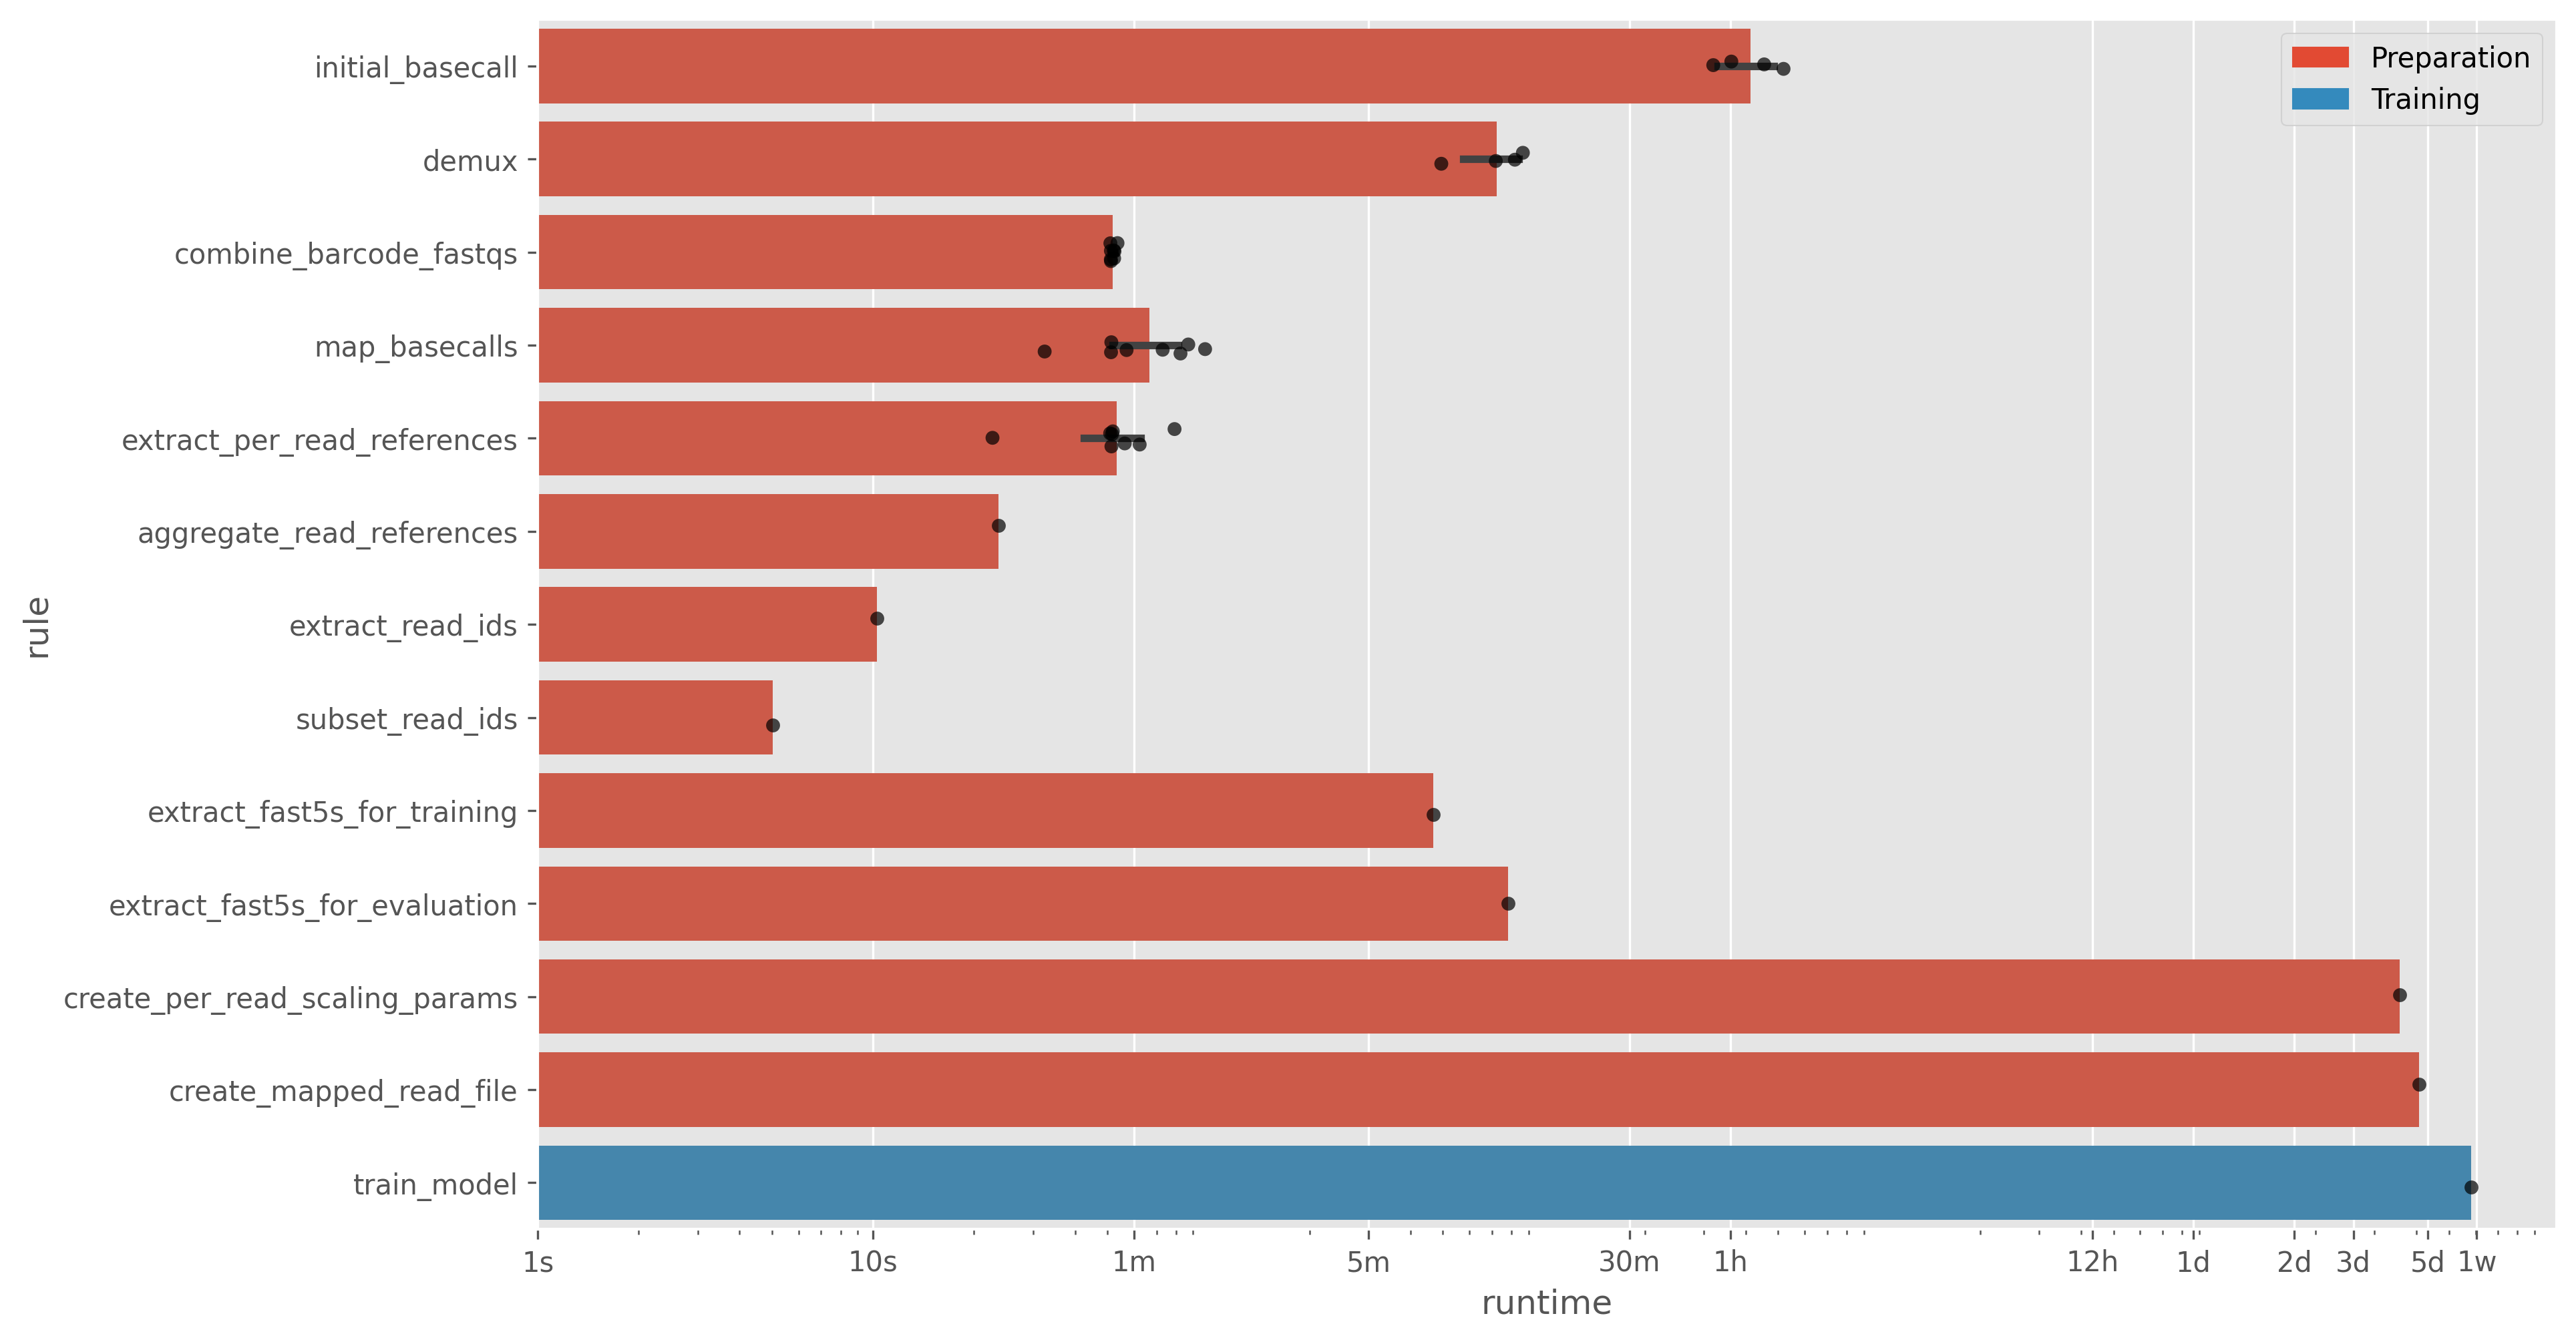
\includegraphics[width=0.9\textwidth]{Chapter4/Figs/prep_runtime.png}
\centering
\caption{Runtimes (x-axis) of the different stages (rules; y-axis) of preparing data for basecall model training (red) and training the model itself (blue). Each individual run is represented with a black point and rules that have multiple runs have black 95\% confidence interval bars. s=seconds; m=minutes; h=hours; d=days; w=weeks.}
\label{fig:prep_runtime}
\end{figure}

\autoref{fig:prep_runtime} shows the runtime of each step in the preparation phase of training. The two longest stages, trimming the raw signal (\vrb{create\_per\_read\_scaling\_params}) and mapping the raw signal to read-references (\vrb{create\_mapped\_read\_file}), took 4.1 and 4.7 days respectively. In total, the full preparation pipeline ran in 8.9 days. 

\subsubsection{Training}

The signal-to-sequencing mapping file produced from the preparation pipeline is the data file used for model training. In addition, we provide an initial model file from which training begins; the mLstm flipflop model distributed with \taiyaki{}.

We train the model using \taiyaki{}'s \vrb{train\_flipflop.py} script with the following parameters: a base layer size of 256; a model stride of 2; a window length over the data of 19; a minimum and maximum length of random training data chunks of 2000 and 4000, respectively; and a maximum learning rate of $0.002\sqrt{g}$, where $g$ is the number of GPUs used for training. The training took 162 hours (6.75 days) to complete on 2 GPUs and had a peak memory usage of 57GB. 

The final output from training the model is a checkpoint file, which we then convert to a \guppy{}-compatible JSON configuration file using \taiyaki{}.

%%%%%%%%%%%%%%%%%%%%%%%%%%%%%%%%%%%%%%%%%%%%%%%%%%%%%%%%%%%%%%%%%%%%%%%%%%%%%%%%%
\section{Evaluating a custom \ont{} basecalling model}

The model-training process produces a JSON file that can be used as a model configuration to basecall \ont{} reads using \guppy{}. The first step in evaluating whether our \mtb{}-specific model, \tubby{}, provides improved accuracy compared to \guppy{}'s default model is to basecall the validation reads that were set aside prior to training. These validation reads provide an unbiased dataset to evaluate on as they were not involved in the training process. 

Although the validation data was not used for training, they are from from the same data source (sample). Therefore, we additionally assess both models on an independent BCG dataset (\autoref{sec:tubby-data}). This BCG sample was not sequenced in the same experiment as the training and validation samples. Additionally, it is a different species (\textit{M. bovis}), but still part of the same genus and the MTBC. As such, it serves as a test of each model's generalisation capabilities. 

We evaluate the read- and consensus-level accuracy of reads produced by \guppy{} and \tubby{} and assess the types of errors made by each. 

% =====
\subsection{Read-level performance}
\label{sec:tubby-read}

The first evaluation metric, read BLAST identity, determines the read-level accuracy produced by the basecalling model. We align the basecalled reads to their respective truth assembly with \vrb{minimap2}, discarding secondary alignments (but keeping unmapped reads). From the resulting pairwise alignment (PAF) file we calculate the BLAST identity as, for each mapping, the number of matching bases divided by the length of the alignment. 

In addition to read BLAST identity, we also assess the relative read lengths produced by each basecalling model. We define relative read length as the length of the aligned part of the read, divided by the total length of the read. The purpose of this metric is to see whether there is a bias towards insertions (greater than 1.0) or deletions (less than 1.0). 

\subsubsection{Validation data}

\autoref{fig:eval-read-blast} shows the distribution of read BLAST identity values for each \guppy{} version and associated \tubby{} model. For all versions, \tubby{} has the highest read BLAST identity values - i.e., distribution of values is tighter, and the mode is further to the right. Interestingly, the best performing version for both models was 3.6.0, with a median BLAST identity of 95.54\% and 94.13\% for \tubby{} and \guppy{} respectively. \autoref{tab:read-blast} describes the summary statistics of the read BLAST identity distributions.

While version 3.6.0 has the highest median values for both models, it is important not to rely on this alone. For instance, version 4.4.0 has the highest minimum value for both models, and the highest mode (\tubby{} version 3.6.0 and 4.4.0 have the same mode). However, the percentiles are highest for version 3.6.0.

\begin{figure}
     \centering
     \begin{subfigure}[b]{0.9\textwidth}
        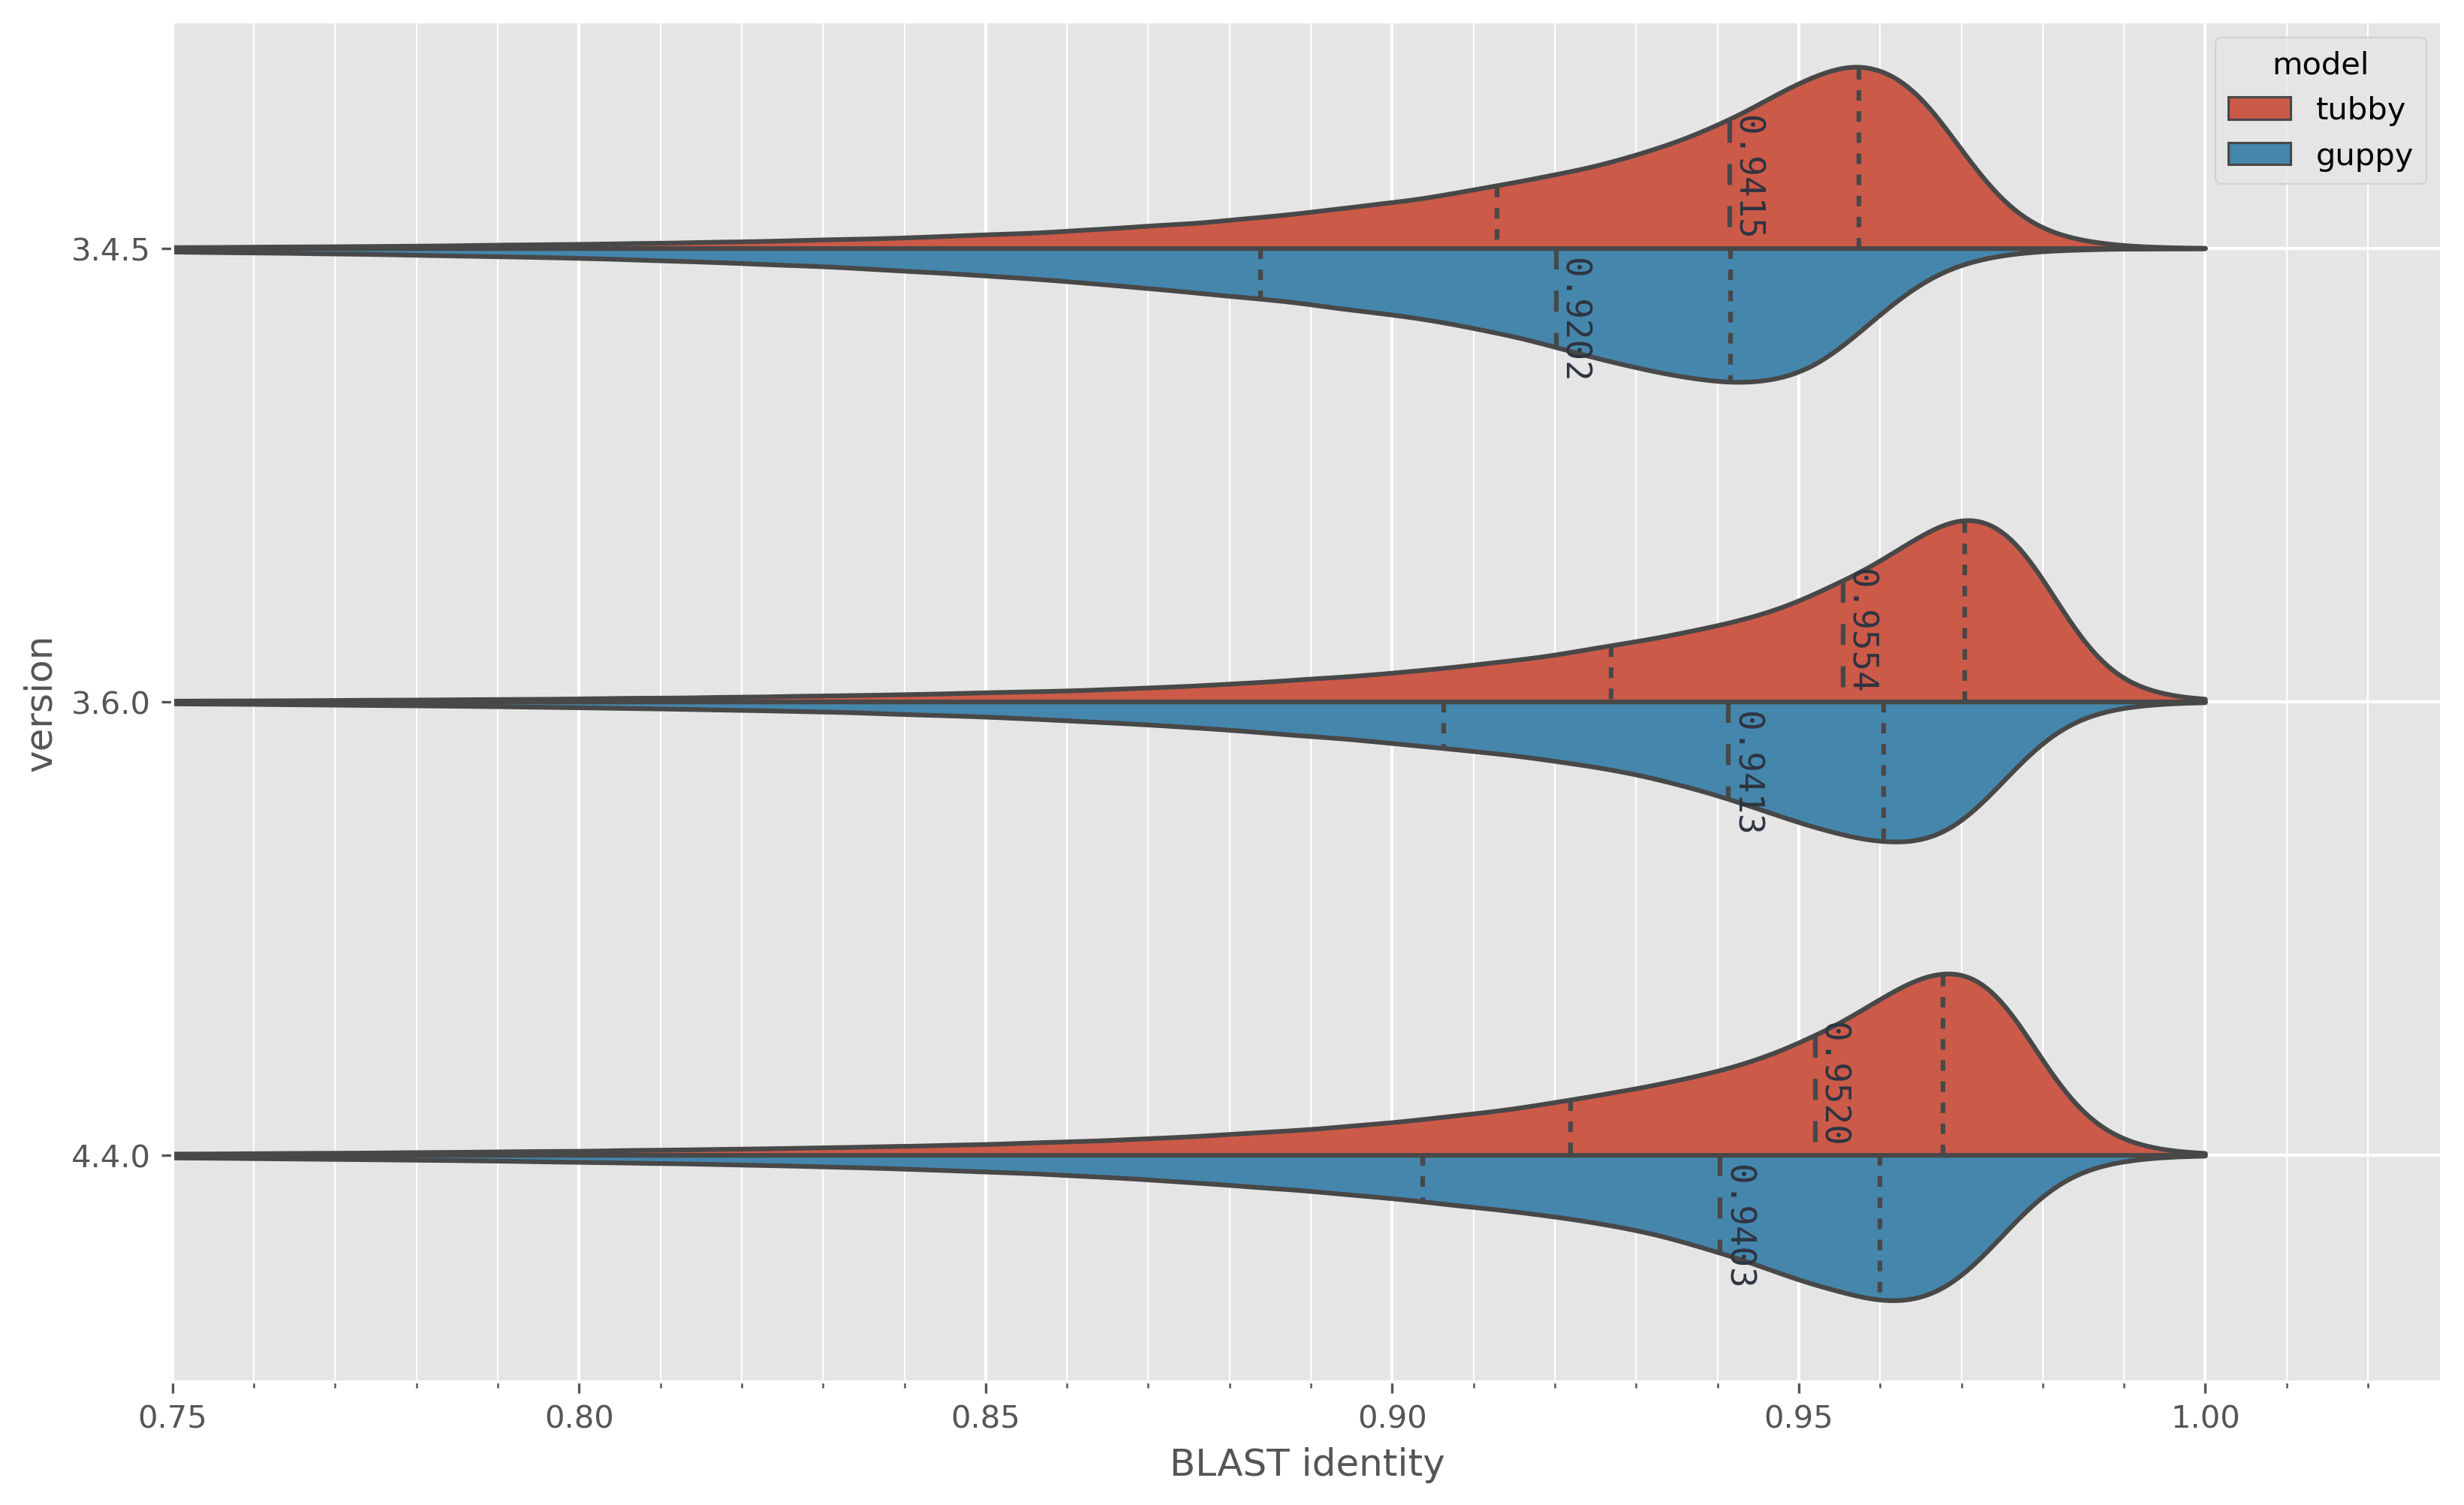
\includegraphics[width=1\linewidth]{Chapter4/Figs/read_blast_identity.png}
        \centering
        \caption{Validation data}
        \label{fig:eval-read-blast}
     \end{subfigure}
     \hfill
     \begin{subfigure}[b]{0.9\textwidth}
         \centering
        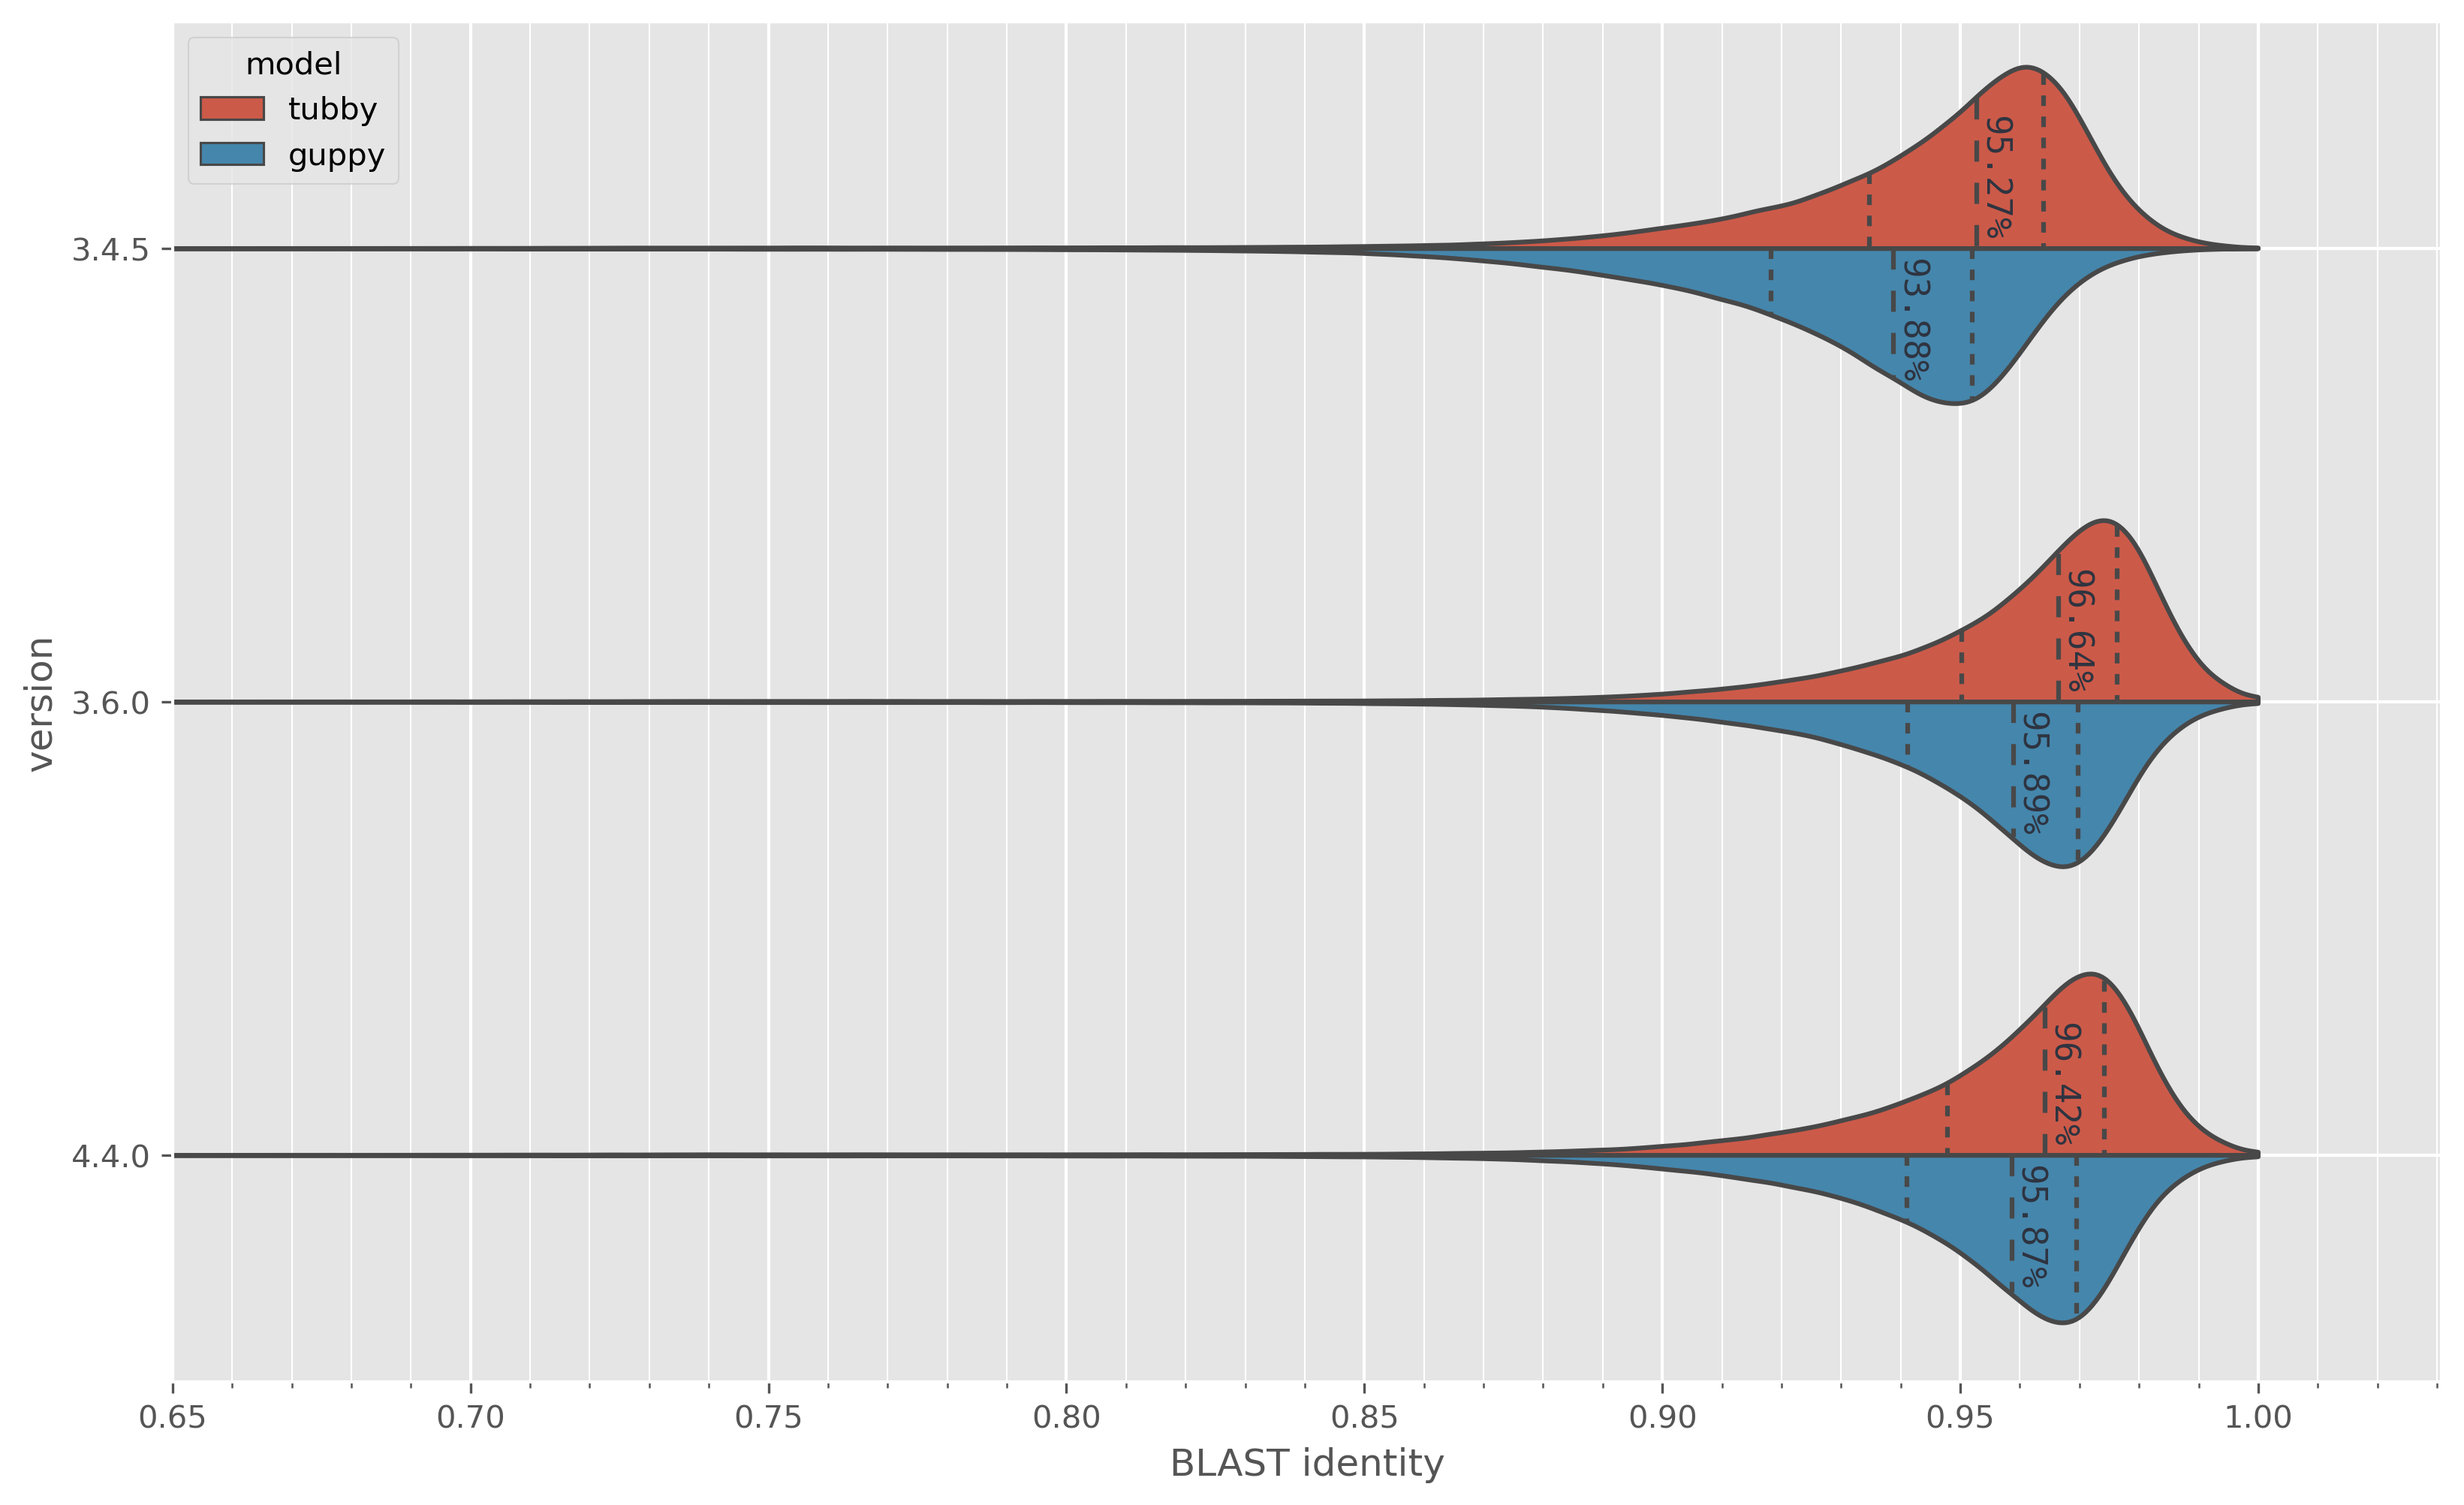
\includegraphics[width=1\linewidth]{Chapter4/Figs/test_read_blast_identity.png}
         \caption{Test data}
         \label{fig:test-read-blast}
     \end{subfigure}
    \caption{Read BLAST identity (x-axis) for the \mtb{}-specific basecalling model \tubby{} (red) compared with the default \guppy{} model (blue). The subtitle of each plot indicates the data being assessed. Version (y-axis) indicates the \guppy{} version used for the basecalling prior to, and after, training. BLAST identity is the number of matching bases (in a read alignment) divided by the length of the alignment. The median value for each violin is annotated on the middle dashed line.}
        \label{fig:read-blast}
\end{figure}

\begin{table}
\centering
\resizebox{\textwidth}{!}{%
\begin{tabular}{@{}llrrrrrrrrr@{}}
\toprule
Version                & Model & Count   & Mean   & std    & Min    & 25\%   & 50\%   & 75\%   & Max    & Mode    \\ \midrule
\multirow{2}{*}{3.4.5} & \guppy{} & 1047829 & 0.9067 & 0.0480 & 0.4186 & 0.8838 & 0.9202 & 0.9416 & 1.0000 & 0.9444 \\
                       & \tubby{} & 1047508 & 0.9295 & \textbf{0.0402} & 0.4619 & 0.9129 & 0.9415 & 0.9574 & 1.0000 & 0.9545 \\
\multirow{2}{*}{3.6.0} & \guppy{} & 1110664 & 0.9268 & 0.0474 & 0.4186 & 0.9063 & 0.9413 & 0.9604 & 1.0000 & 0.9615 \\
                       & \tubby{} & 1110098 & \textbf{0.9423} & 0.0413 & 0.4297 & \textbf{0.9269} & \textbf{0.9554} & \textbf{0.9704} & 1.0000 & \textbf{0.9688} \\
\multirow{2}{*}{4.4.0} & \guppy{} & 1144426 & 0.9247 & 0.0496 & \textbf{0.4751} & 0.9038 & 0.9403 & 0.9600 & 1.0000 & 0.9628 \\
                       & \tubby{} & 1143410 & 0.9381 & 0.0435 & 0.4723 & 0.9220 & 0.9520 & 0.9678 & 1.0000 & \textbf{0.9688} \\ \cmidrule(l){2-11} 
\end{tabular}%
}
\caption{Read BLAST identity summary statistics for the \mtb{}-specific basecalling model \tubby{} compared with the default \guppy{} model on the validation data. Version indicates the \guppy{} version used for the basecalling prior to, and after, training. BLAST identity is the number of matching bases (in a read alignment) divided by the length of the alignment. Count refers to the number of reads evaluated. std=standard deviation.}
\label{tab:read-blast}
\end{table}

\autoref{fig:eval-read-rel-len} shows that \tubby{} has a slight tendency towards deletions (shorter reads) compared to \guppy{}. However, this result is a little more complex than just looking at median values. The distribution of lengths for \guppy{} extends much further past 1.0 compared with \tubby{}, indicating an increase in insertions. We will return to this result when we look at the error types (\autoref{sec:tubby-error-types}). Summary statistics for the relative read lengths are shown in \autoref{tab:read-rel-len}.

\begin{figure}
     \centering
     \begin{subfigure}[b]{0.9\textwidth}
        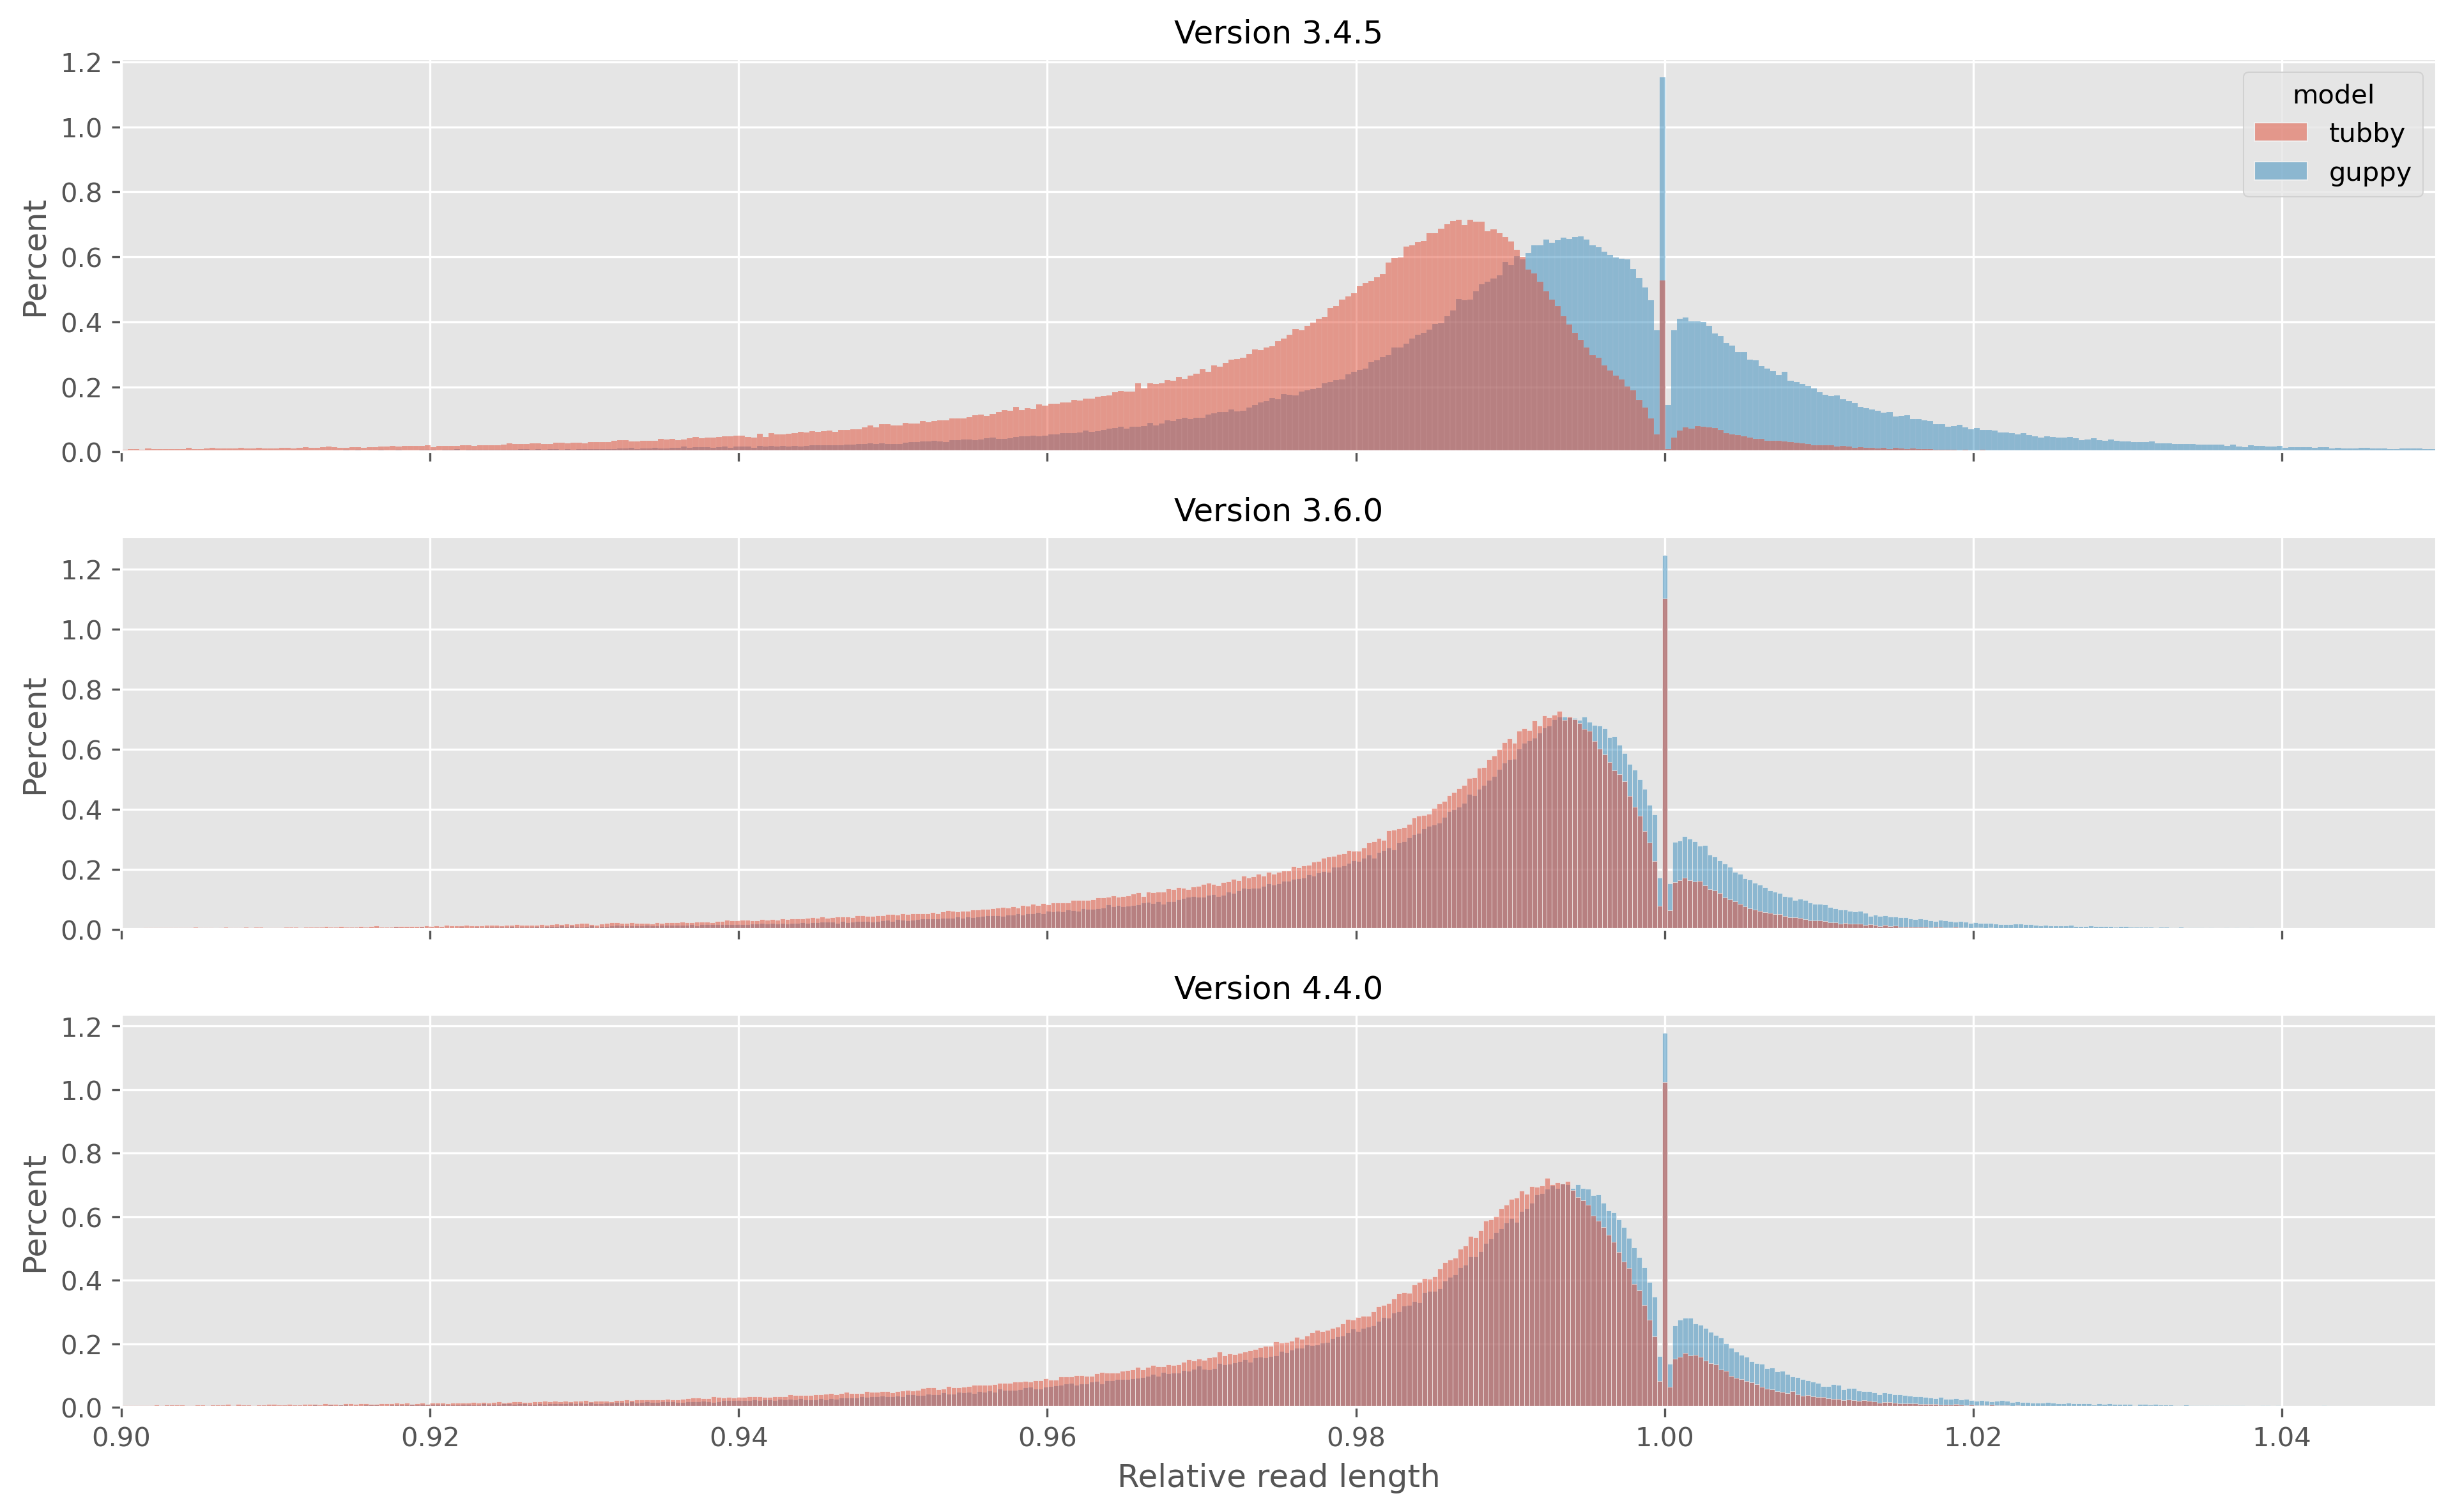
\includegraphics[width=1\linewidth]{Chapter4/Figs/read_rel_len.png}
        \centering
        \caption{Validation data}
        \label{fig:eval-read-rel-len}
     \end{subfigure}
     \hfill
     \begin{subfigure}[b]{0.9\textwidth}
         \centering
        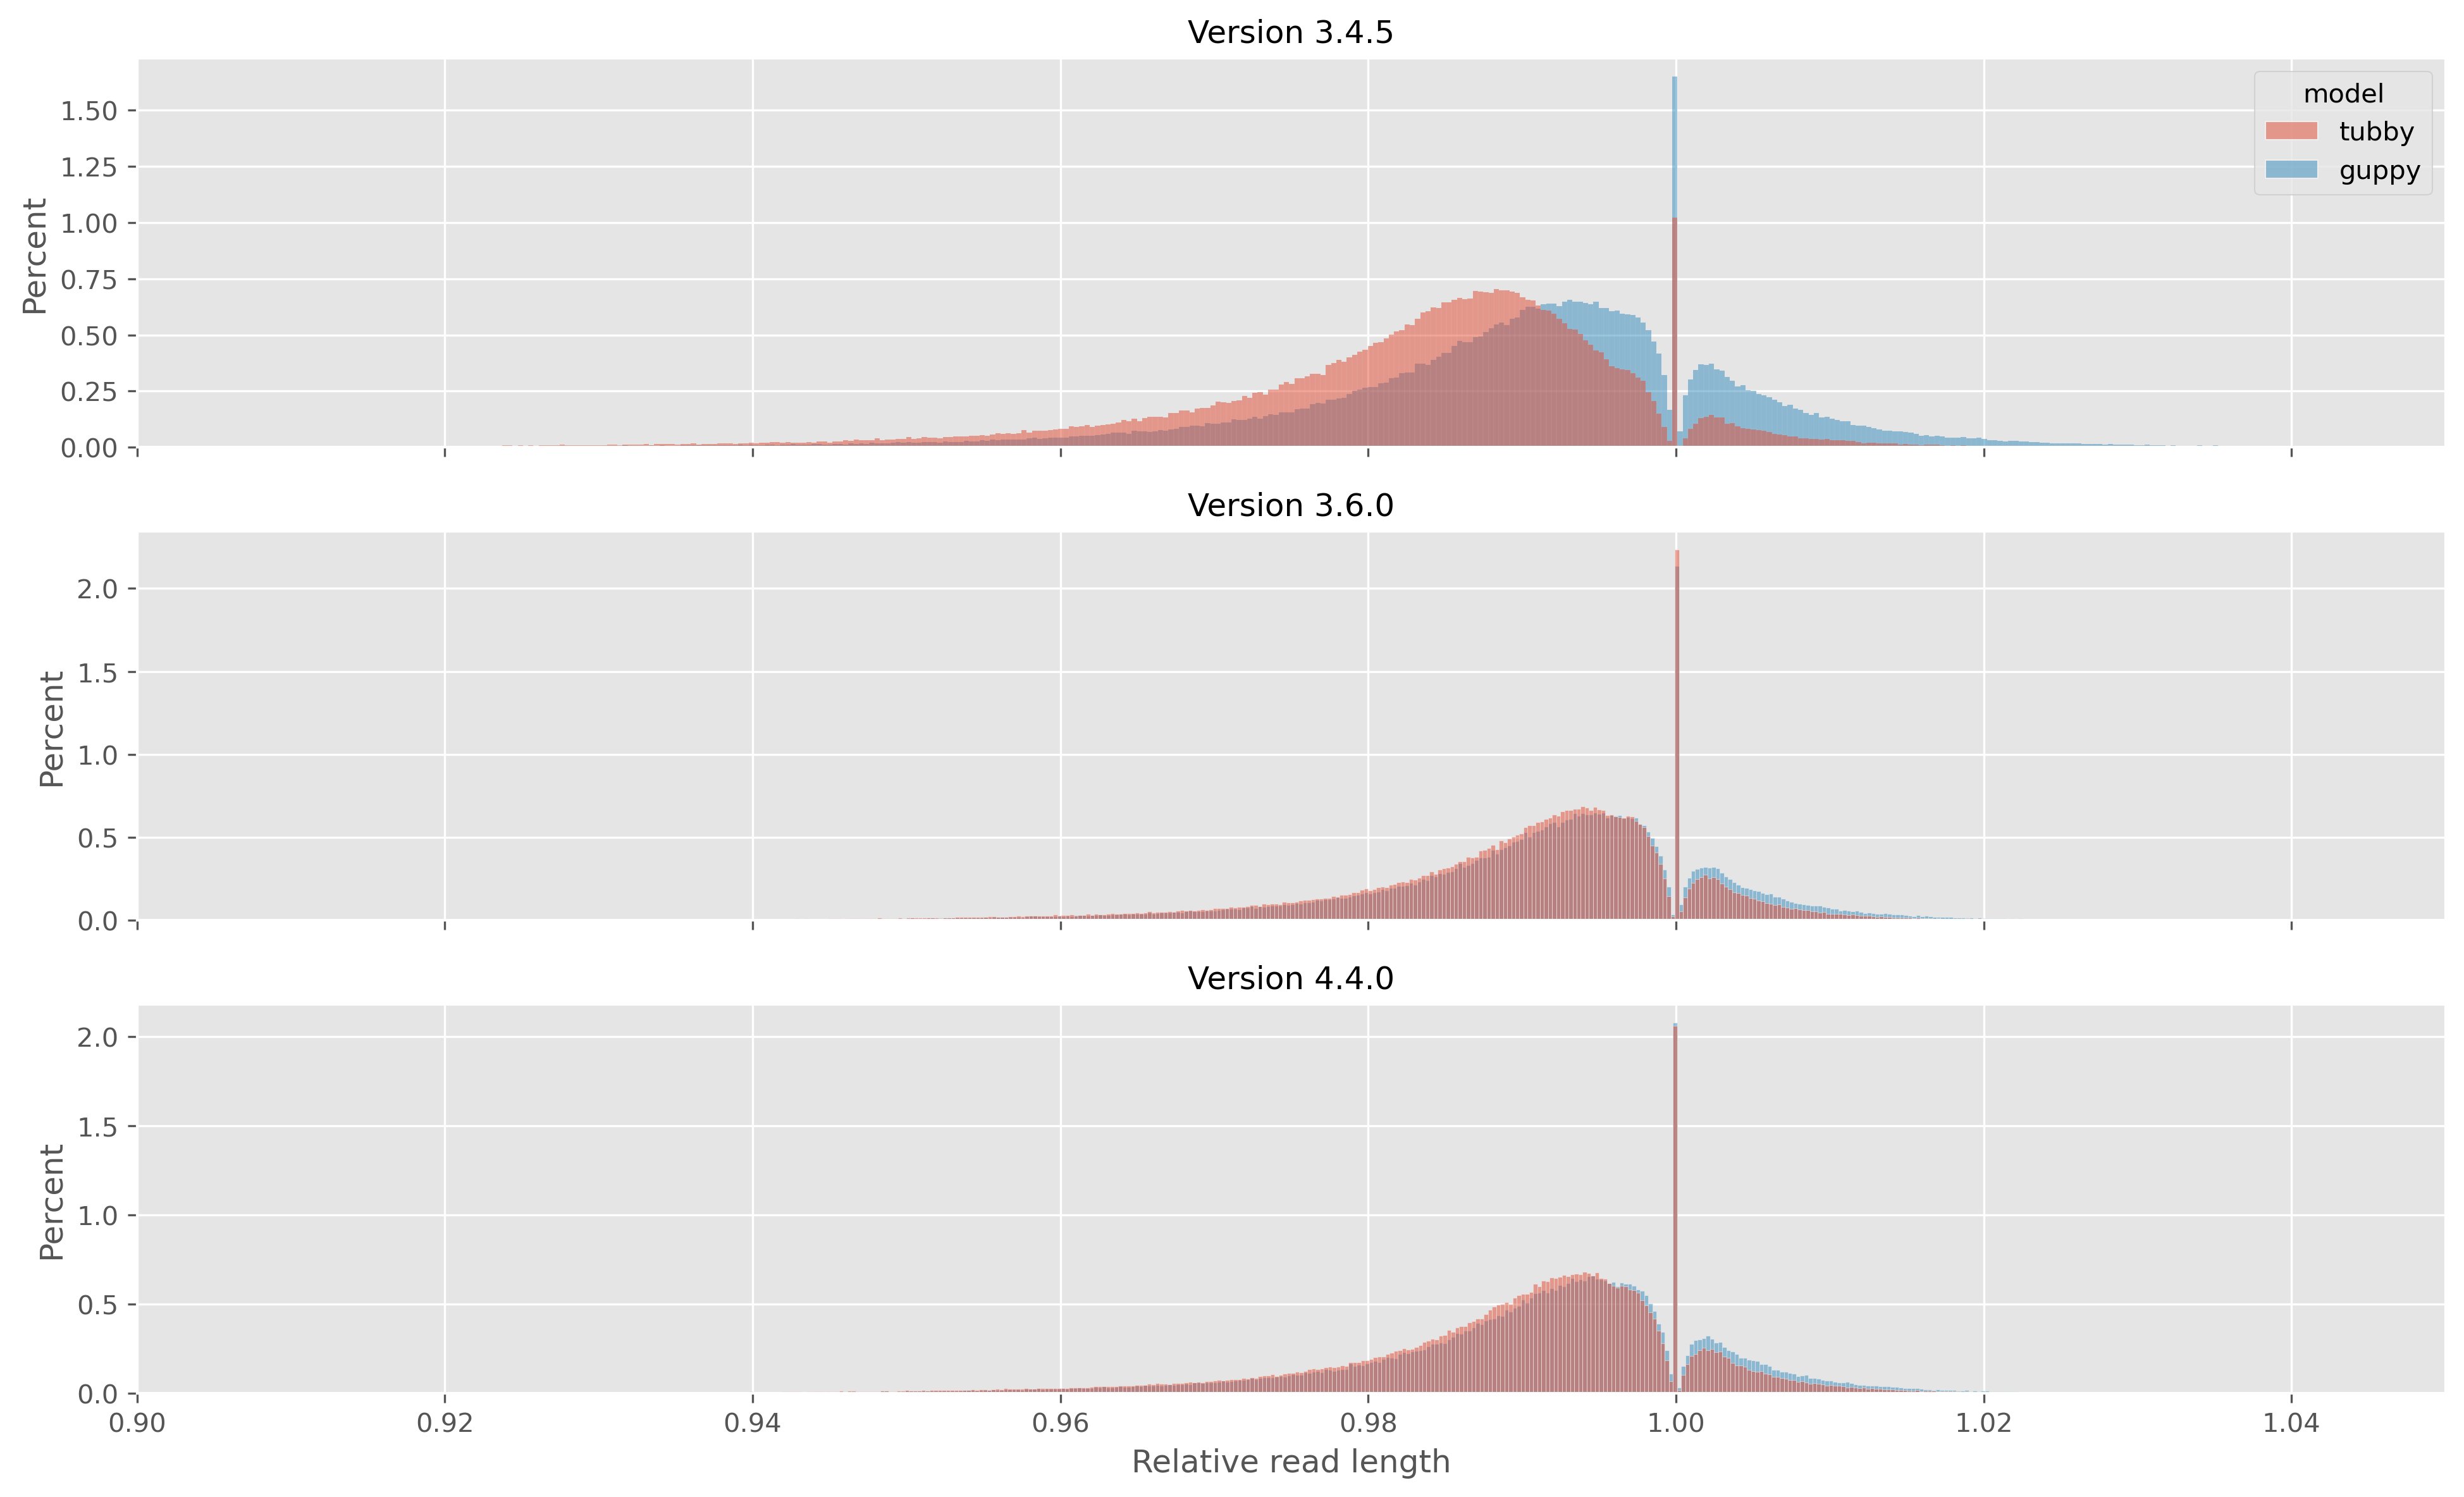
\includegraphics[width=1\linewidth]{Chapter4/Figs/test_read_rel_len.png}
         \caption{Test data}
         \label{fig:test-read-rel-len}
     \end{subfigure}
        \caption{Relative read length (y-axis) for the \mtb{}-specific basecalling model \tubby{} (red) compared with the default \guppy{} model (blue). The subtitle of each plot indicates the data being assessed. Relative read length is the length of the aligned part of the read, divided by the total length of the read. Version indicates the \guppy{} version used for the basecalling prior to, and after, training.}
        \label{fig:read-rel-len}
\end{figure}

\begin{table}
\centering
\resizebox{\textwidth}{!}{%
\begin{tabular}{@{}llrrrrrrrr@{}}
\toprule
Version                & Model & Count   & Mean   & std    & Min    & 25\%   & 50\%   & 75\%   & Max    \\ \midrule
\multirow{2}{*}{3.4.5} & \guppy{} & 1047829 & 0.9919 & 0.0240 & 0.4558 & 0.9842 & 0.9932 & 1.0014 & 1.9881 \\
                       & \tubby{} & 1047508 & 0.9764 & 0.0239 & 0.4936 & 0.9698 & 0.9822 & 0.9892 & 1.8949 \\
\multirow{2}{*}{3.6.0} & \guppy{} & 1110664 & 0.9873 & 0.0233 & 0.4495 & 0.9819 & 0.9914 & 0.9974 & 2.0322 \\
                       & \tubby{} & 1110098 & 0.9817 & 0.0241 & 0.4531 & 0.9761 & 0.9882 & 0.9943 & 1.9031 \\
\multirow{2}{*}{4.4.0} & \guppy{} & 1144426 & 0.9862 & 0.0241 & 0.5085 & 0.9806 & 0.9907 & 0.9969 & 1.9146 \\
                       & \tubby{} & 1143410 & 0.9814 & 0.0246 & 0.4963 & 0.9758 & 0.9879 & 0.9941 & 1.8851 \\ \cmidrule(l){2-10} 
\end{tabular}%
}
\caption{Relative read length for the \mtb{}-specific basecalling model \tubby{} compared with the default \guppy{} model on the validation data. Relative read length is the length of the aligned part of the read, divided by the total length of the read. Version indicates the \guppy{} version used for the basecalling prior to, and after, training. Count refers to the number of reads evaluated. std=standard deviation.}
\label{tab:read-rel-len}
\end{table}

\subsubsection{Test data}

\autoref{fig:test-read-blast} shows the read BLAST identities for the test BCG sample. As with the validation data, version 3.6.0 \tubby{} has the highest median read identity of 96.64\% - 1.10\% greater than the validation data. From \autoref{tab:test-read-blast}, we see that \tubby{} version 3.6.0 has the highest percentiles, mode (97.67\%), and mean (95.87\%) of all the models and versions.

Again, for each version, \tubby{} outperforms \guppy{} on all summary statistics (except the mode for version 4.4.0, which is the same).

\begin{table}
\centering
\resizebox{\textwidth}{!}{%
\begin{tabular}{@{}llrrrrrrrrr@{}}
\toprule
Version                & Model & Count   & Mean   & std    & Min    & 25\%   & 50\%   & 75\%   & Max    & Mode    \\ \midrule
\multirow{2}{*}{3.4.5} & \guppy{} & 787170 & 0.9309 & 0.0330          & 0.4738 & 0.9183 & 0.9388 & 0.9520 & 1.0000 & 0.9444 \\
                       & \tubby{} & 790230 & 0.9453 & 0.0308          & 0.4764 & 0.9348 & 0.9527 & 0.9640 & 1.0000 & 0.9545 \\
\multirow{2}{*}{3.6.0} & \guppy{} & 791527 & 0.9509 & 0.0321          & 0.3841 & 0.9412 & 0.9589 & 0.9698 & 1.0000 & 0.9688 \\
 & \tubby{} & 791356 & \textbf{0.9587} & 0.0307 & \textbf{0.4819} & \textbf{0.9502} & \textbf{0.9664} & \textbf{0.9763} & 1.0000 & \textbf{0.9767} \\
\multirow{2}{*}{4.4.0} & \guppy{} & 790291 & 0.9507 & 0.0318          & 0.4328 & 0.9411 & 0.9587 & 0.9695 & 1.0000 & 0.9688 \\
                       & \tubby{} & 791217 & 0.9566 & \textbf{0.0305} & 0.3915 & 0.9479 & 0.9642 & 0.9742 & 1.0000 & 0.9688 \\ \cmidrule(l){2-11} 
\end{tabular}%
}
\caption{Read BLAST identity summary statistics for the \mtb{}-specific basecalling model \tubby{} compared with the default \guppy{} model on the test data. Version indicates the \guppy{} version used for the basecalling prior to, and after, training. BLAST identity is the number of matching bases (in a read alignment) divided by the length of the alignment. Count refers to the number of reads evaluated. std=standard deviation.}
\label{tab:test-read-blast}
\end{table}

The relative read length distributions show in \autoref{fig:test-read-rel-len} indicate that on the test data, \tubby{} and \guppy{} have the same slight tendency towards deletions (shorter reads). However, both models have much similar relative read lengths to each other when compared to the validation data - except version 3.4.5. Summary statistics for the relative read lengths are shown in \autoref{tab:test-read-rel-len}.

\begin{table}
\centering
\resizebox{\textwidth}{!}{%
\begin{tabular}{@{}llllllllll@{}}
\toprule
Version                & Model & Count   & Mean   & std    & Min    & 25\%   & 50\%   & 75\%   & Max    \\ \midrule
\multirow{2}{*}{3.4.5} & \guppy{} & 787170 & 0.990146 & 0.020453 & 0.507716 & 0.983563 & 0.991832 & 0.998854 & 1.885660 \\
                       & \tubby{} & 790230 & 0.982657 & 0.020303 & 0.512180 & 0.976847 & 0.985492 & 0.991870 & 2.011945 \\
\multirow{2}{*}{3.6.0} & \guppy{} & 791527 & 0.990858 & 0.019202 & 0.516049 & 0.986090 & 0.993108 & 0.998485 & 2.519333 \\
                       & \tubby{} & 791356 & 0.989297 & 0.019148 & 0.519136 & 0.984899 & 0.992054 & 0.997132 & 2.017065 \\
\multirow{2}{*}{4.4.0} & \guppy{} & 790291 & 0.990601 & 0.019214 & 0.515123 & 0.985816 & 0.992832 & 0.998220 & 2.137884 \\
                       & \tubby{} & 791217 & 0.989091 & 0.019307 & 0.514339 & 0.984615 & 0.991718 & 0.996894 & 2.525117 \\ \cmidrule(l){2-10} 
\end{tabular}%
}
\caption{Relative read length for the \mtb{}-specific basecalling model \tubby{} compared with the default \guppy{} model on the test data. Relative read length is the length of the aligned part of the read, divided by the total length of the read. Version indicates the \guppy{} version used for the basecalling prior to, and after, training. Count refers to the number of reads evaluated. std=standard deviation.}
\label{tab:test-read-rel-len}
\end{table}

% =====
\subsection{Consensus-level performance}

To assess consensus-level accuracy of each model, we require assemblies from the basecalled reads. However, to allow for comparison of these model-specific consensus sequences (assemblies) to the truth assembly, a reference-guided method is needed to ensure overall structure of the truth and consensus sequences is the same. We use Rebaler (version 0.2.0; \url{https://github.com/rrwick/Rebaler}), a tool developed for exactly this use-case \cite{wick2019}. Briefly, \vrb{rebaler} aligns the reads to a reference sequence and replaces that sequence with the sequence from the best alignments, producing an unpolished assembly. After this, it polishes the assembly with \vrb{racon} to produce a consensus sequence. 

We evaluate consensus accuracy in two ways. In the first, we use the same approach as in \cite{wick2020} to quantify the similarity of the consensus and truth assemblies for each sample. Each contig (chromosome) in the consensus assembly in aligned to the truth assembly with \vrb{minimap2}. We calculate the chromosome identity for each contig's longest alignment in the same fashion as BLAST identity (\autoref{sec:tubby-read}). Second, in the same manner as \cite{wick2019}, we cut the consensus assembly into 10kbp chunks - simulating consensus "reads" - and align these to the truth assembly to calculate the BLAST identity. 

\subsubsection{Validation data}

\autoref{fig:eval-chrom-identity} shows the chromosome identity for each version and model. We again see that \tubby{} version 3.6.0 leads to the highest identity values, with a median chromosome identity value of 99.96\%. Compared to the best median \guppy{} identity of 99.94\% (version 3.6.0), \tubby{} provides an improvement of 0.02\%, which equates to approximately 880 less erroneous positions in the \mtb{} assembly.

\begin{figure}
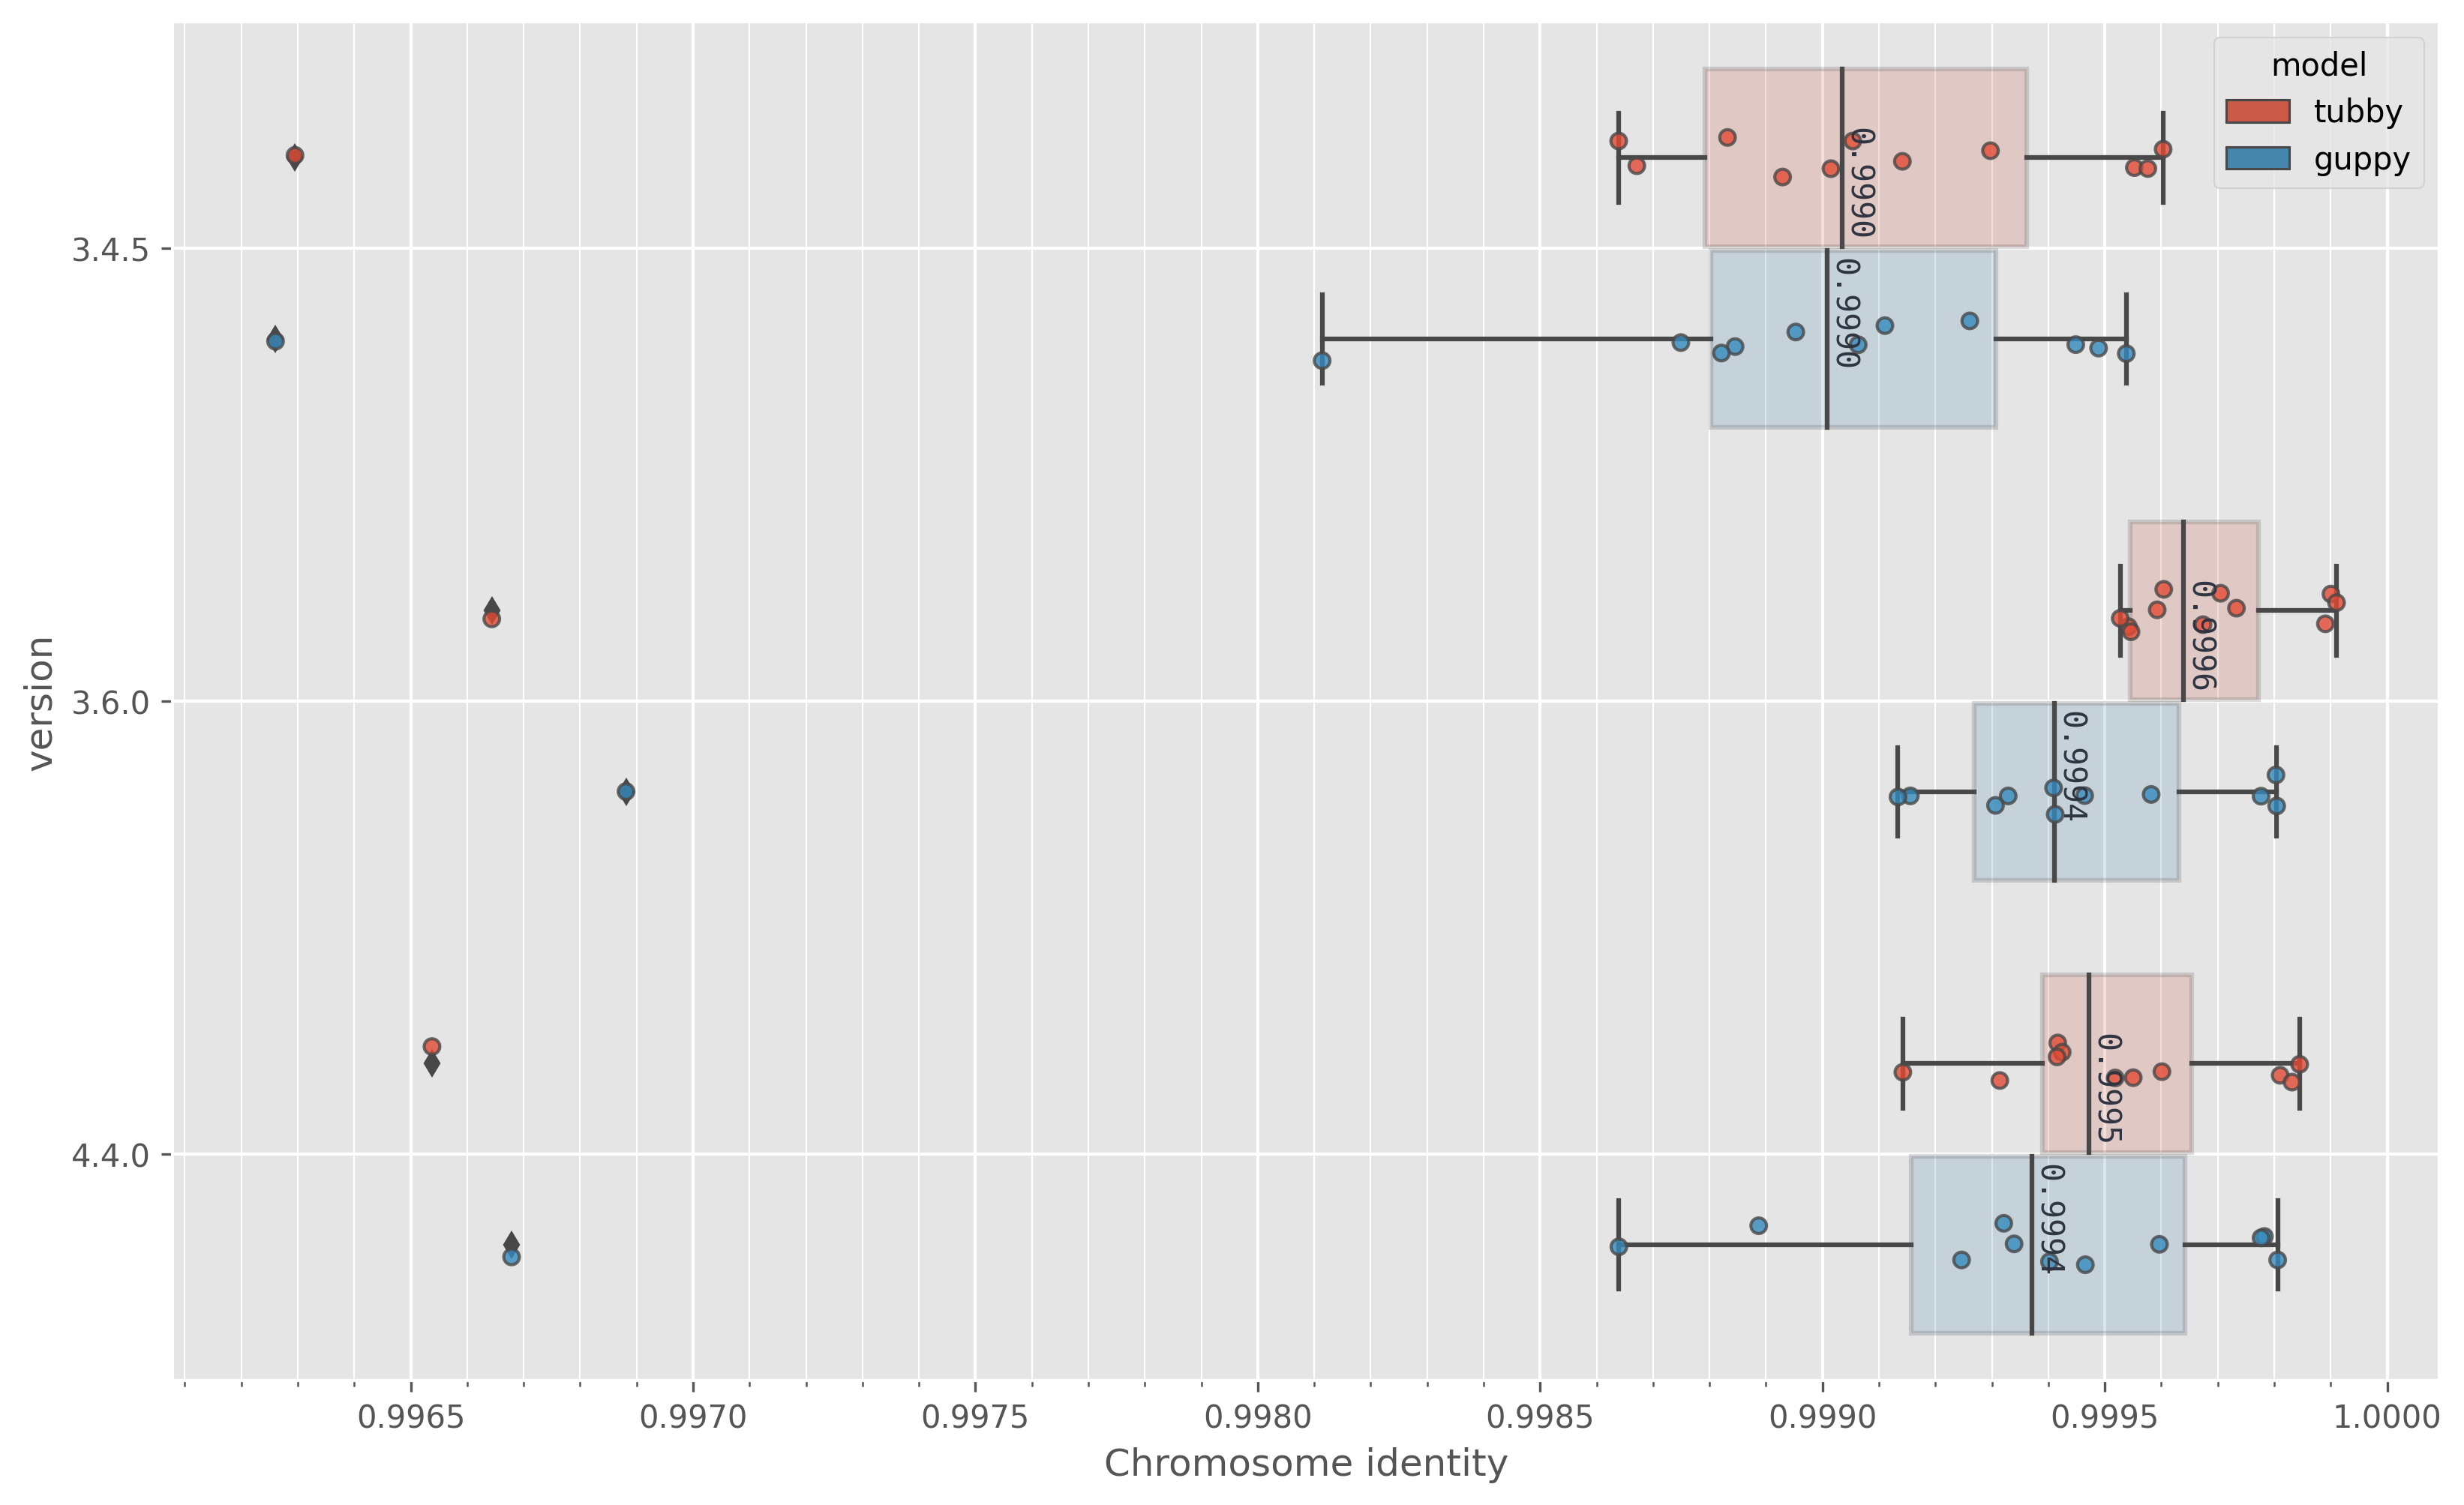
\includegraphics[width=0.9\textwidth]{Chapter4/Figs/eval_chromosome_identity.png}
\centering
\caption{Chromosome identity (x-axis) for the \mtb{}-specific basecalling model \tubby{} (red) compared with the default \guppy{} model (blue) on the validation data. Version (y-axis) indicates the \guppy{} version used for the basecalling prior to, and after, training. For each chromosome's longest alignment to its truth assembly, chromosome identity is the number of matching bases divided by the length of the alignment. The coloured points indicate the individual chromosome identity for each contig in each sample.}
\label{fig:eval-chrom-identity}
\end{figure}

\begin{table}
\centering
\resizebox{\textwidth}{!}{%
\begin{tabular}{@{}llrrrrrrrr@{}}
\toprule
Version                & Model & Contigs & Mean   & std    & Min    & 25\%   & 50\%   & 75\%   & Max    \\ \midrule
\multirow{2}{*}{3.4.5} & \guppy{} & 12      & 0.9988 & 0.0009 & 0.9963 & 0.9988 & 0.9990 & 0.9993 & 0.9995 \\
                       & \tubby{} & 12      & 0.9989 & 0.0009 & 0.9963 & 0.9988 & 0.9990 & 0.9994 & 0.9996 \\
\multirow{2}{*}{3.6.0} & \guppy{} & 12      & 0.9993 & \textbf{0.0008} & \textbf{0.9969} & 0.9993 & 0.9994 & 0.9996 & 0.9998 \\
                       & \tubby{} & 12      & \textbf{0.9994} & 0.0009 & 0.9966 & \textbf{0.9995} & \textbf{0.9996} & \textbf{0.9998} & \textbf{0.9999} \\
\multirow{2}{*}{4.4.0} & \guppy{} & 12      & 0.9992 & 0.0009 & 0.9967 & 0.9992 & 0.9994 & 0.9996 & 0.9998 \\
                       & \tubby{} & 12      & 0.9993 & 0.0009 & 0.9965 & 0.9994 & 0.9995 & 0.9997 & 0.9998 \\ \cmidrule(l){2-10} 
\end{tabular}%
}
\caption{Chromosome identity summary statistics for the \mtb{}-specific basecalling model \tubby{} compared with the default \guppy{} model on the validation data. Version indicates the \guppy{} version used for the basecalling prior to, and after, training. For each chromosome's longest alignment to its truth assembly, chromosome identity is the number of matching bases divided by the length of the alignment. std=standard deviation.}
\label{tab:eval-chrom-identity}
\end{table}

\autoref{fig:eval-consensus-blast} shows \tubby{} version 3.6.0 has a higher median consensus BLAST identity (99.98\%) compared with the best \guppy{} version (0.9997; v4.4.0). The consensus accuracy improvement of 0.0001 equates to approximately 440 less erroneous positions in the \mtb{} assembly. Summary statistics are shown in \autoref{tab:eval-consensus-blast}.

\begin{figure}
     \centering
     \begin{subfigure}[b]{0.9\textwidth}
        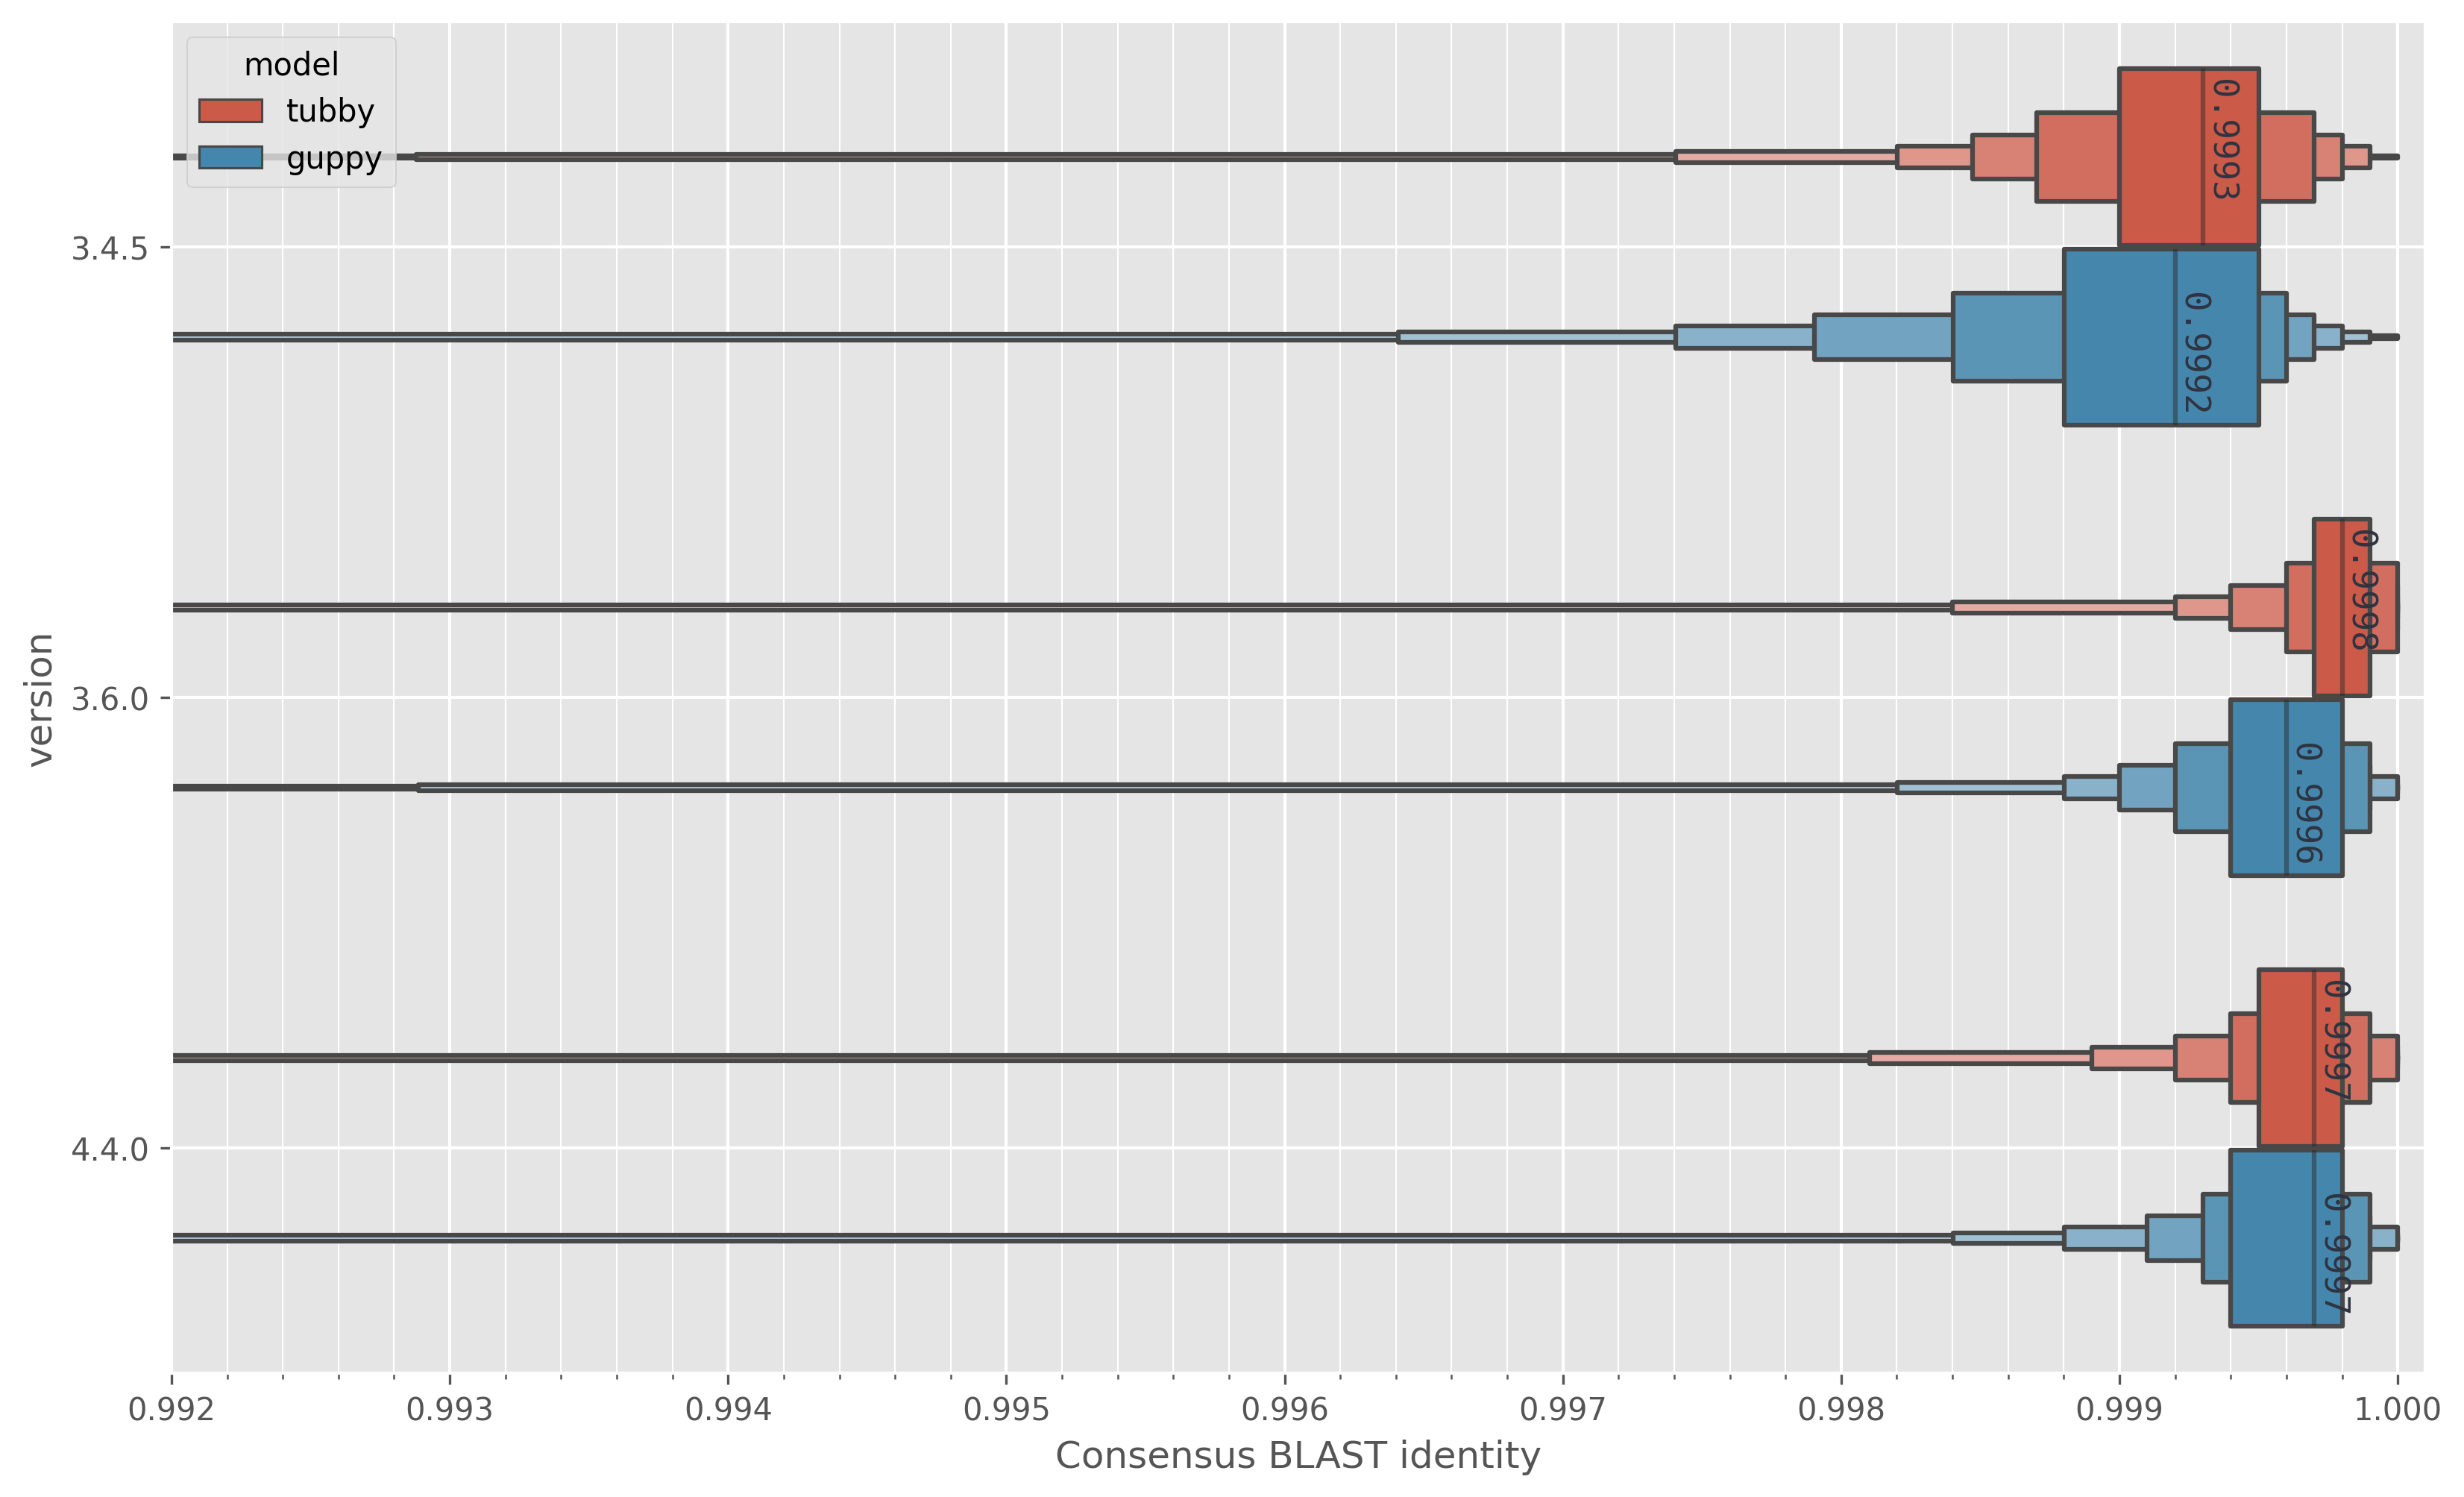
\includegraphics[width=1\linewidth]{Chapter4/Figs/eval_consensus_blast_identity.png}
        \centering
        \caption{Validation data}
        \label{fig:eval-consensus-blast}
     \end{subfigure}
     \hfill
     \begin{subfigure}[b]{0.9\textwidth}
         \centering
        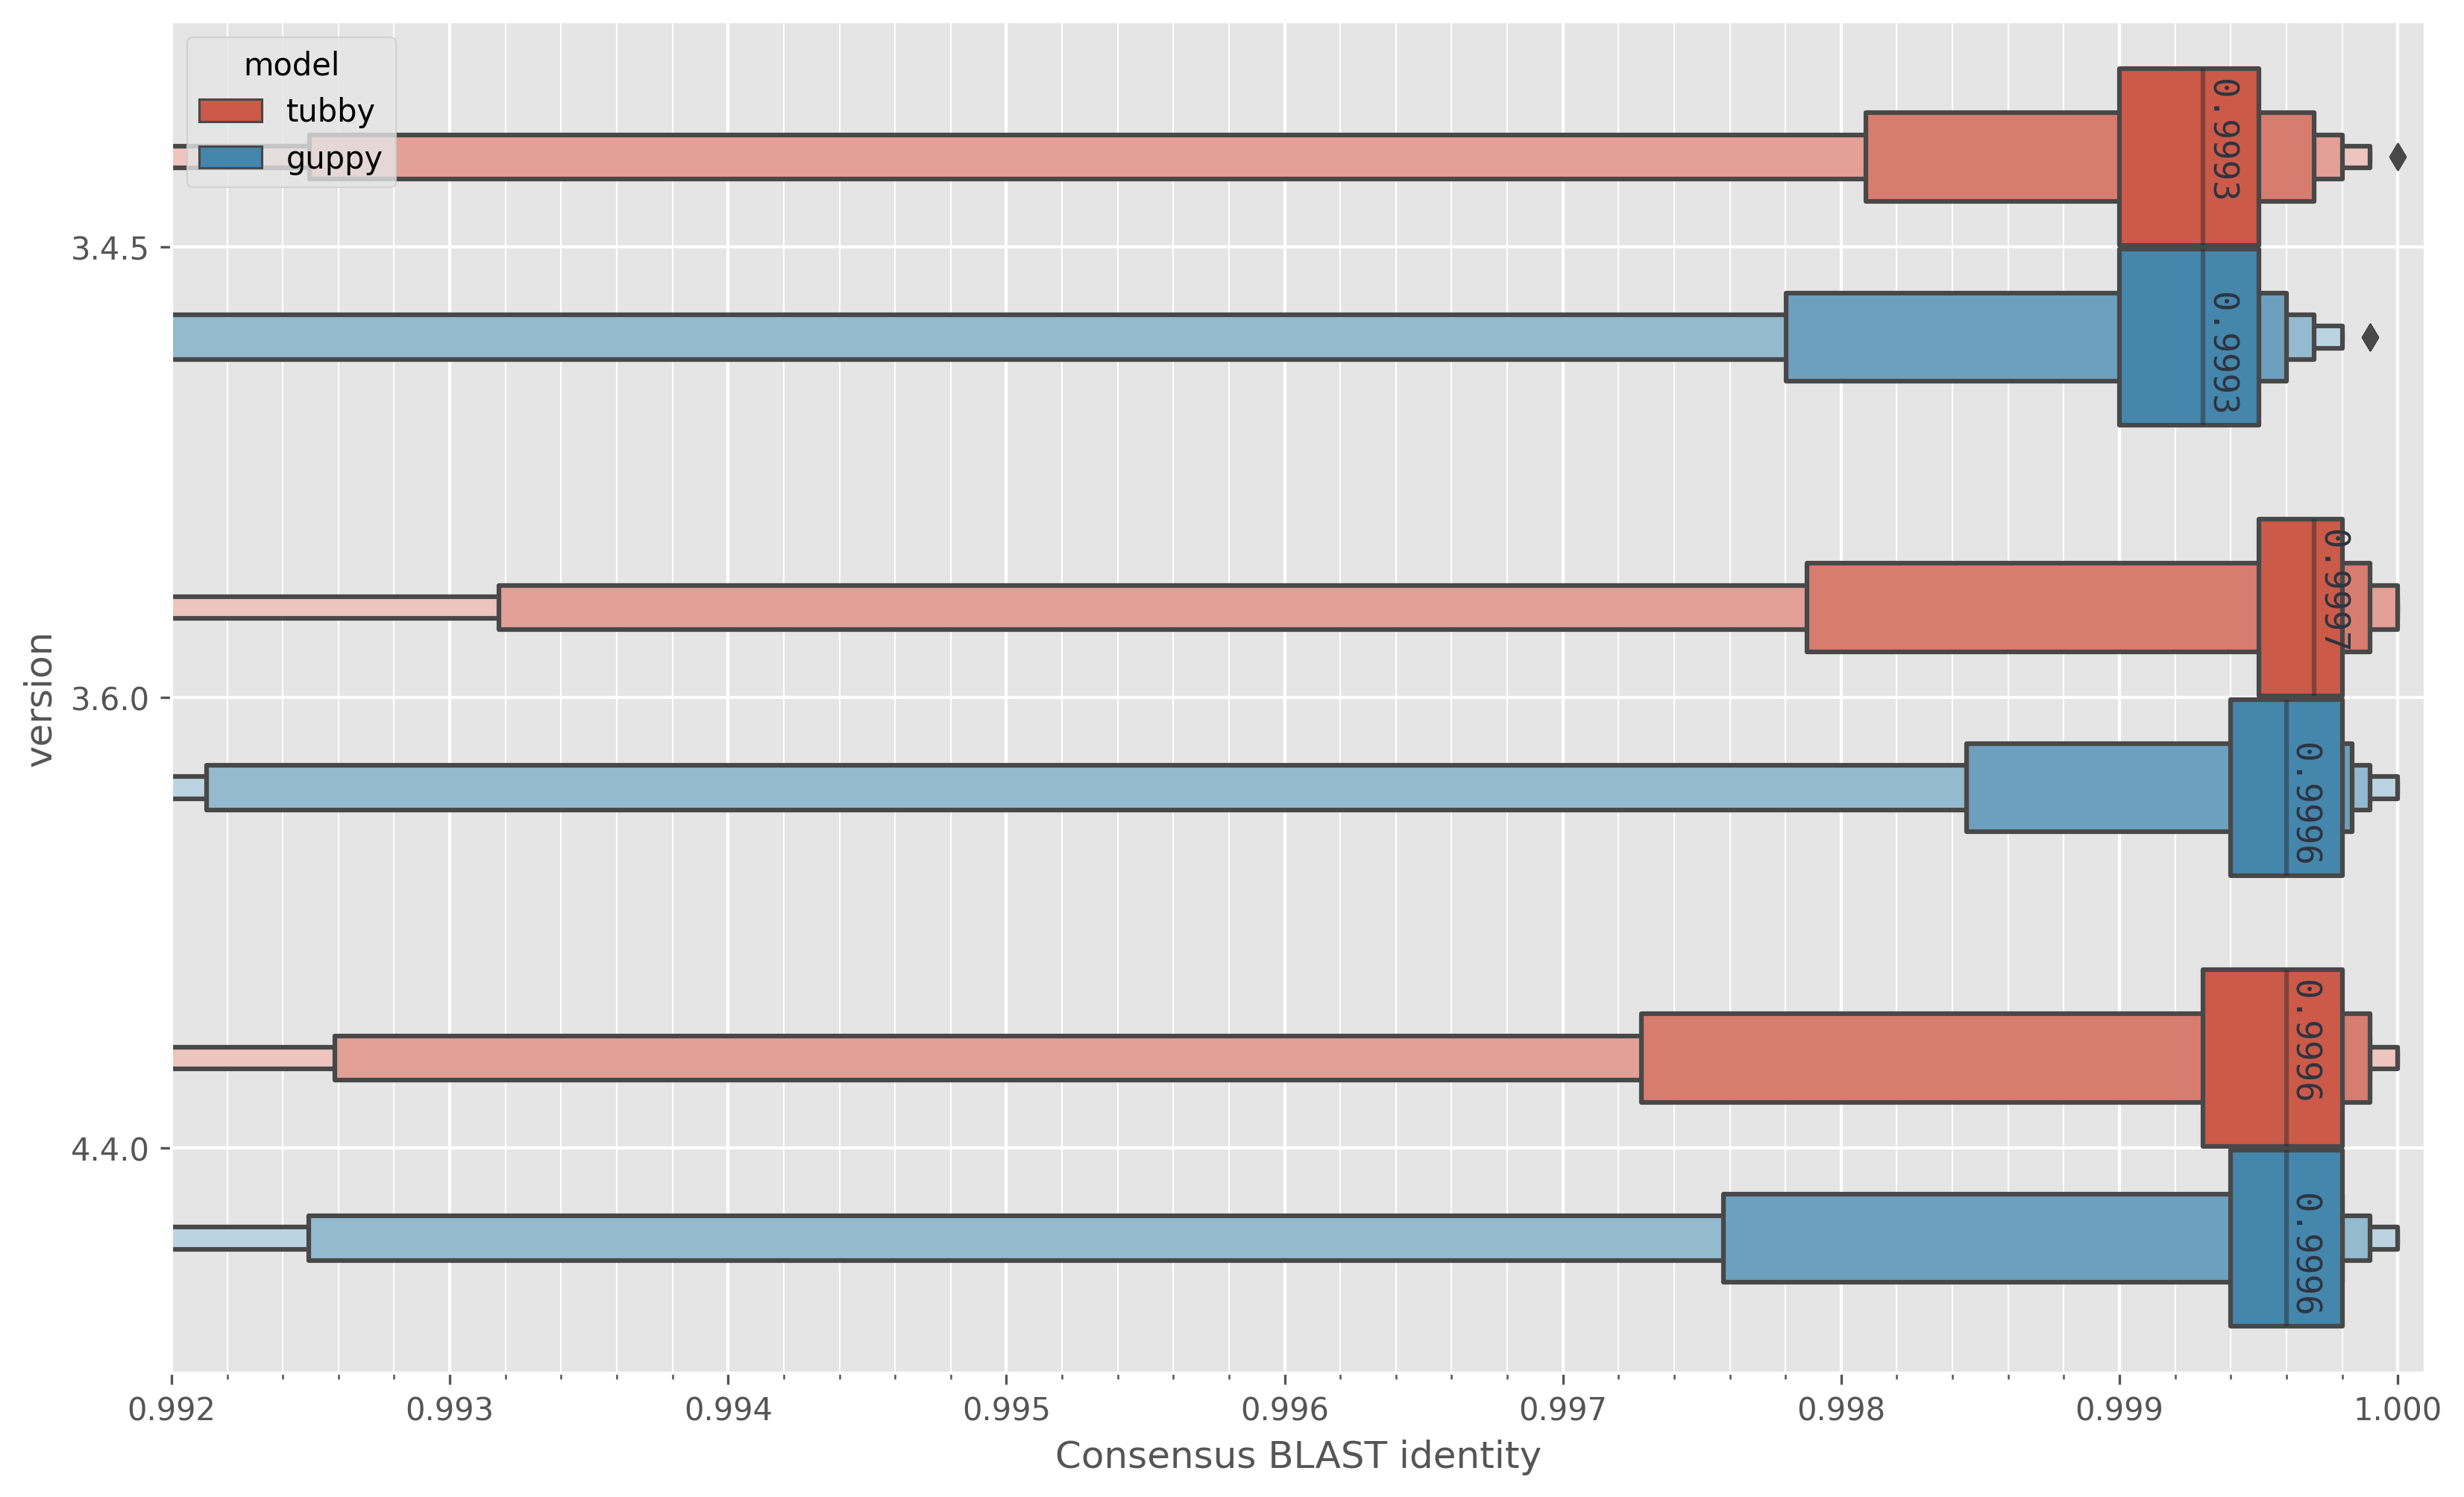
\includegraphics[width=1\linewidth]{Chapter4/Figs/test_consensus_blast_identity.png}
         \caption{Test data}
         \label{fig:test-consensus-blast}
     \end{subfigure}
        \caption{Consensus BLAST identity (Y-axis), where consensus refers to 10kbp "chunks" of the genome assembly produced by the basecalled reads, for each model (colours), mapped to the truth genome. The subtitle of each plot indicates the data being assessed. Version (y-axis) indicates the \guppy{} version used for the basecalling prior to, and after, training. BLAST identity is the number of matching bases (in a chunk alignment) divided by the length of the alignment. The median value for each boxplot is annotated on the middle line.}
        \label{fig:consensus-blast}
\end{figure}

\begin{table}
\centering
\resizebox{\textwidth}{!}{%
\begin{tabular}{@{}llrrrrrrrr@{}}
\toprule
Version                & Model & Contigs & Mean   & std    & Min    & 25\%   & 50\%   & 75\%   & Max    \\ \midrule
\multirow{2}{*}{3.4.5} & \guppy{} & 3531  & 0.9987          & \textbf{0.0044} & \textbf{0.8635} & 0.9988          & 0.9992          & 0.9995          & 1.0000 \\
                       & \tubby{} & 3532  & 0.9990          & 0.0041 & 0.8630          & 0.9990          & 0.9993          & 0.9995          & 1.0000 \\
\multirow{2}{*}{3.6.0} & \guppy{} & 3532  & 0.9993          & 0.0041 & \textbf{0.8635} & 0.9994          & 0.9996          & 0.9998          & 1.0000 \\
                       & \tubby{} & 3534  & \textbf{0.9995} & 0.0043          & 0.8634          & \textbf{0.9997} & \textbf{0.9998} & \textbf{0.9999} & 1.0000 \\
\multirow{2}{*}{4.4.0} & \guppy{} & 3531  & 0.9992          & 0.0058          & 0.7961          & 0.9994          & 0.9997          & 0.9998          & 1.0000 \\
                       & \tubby{} & 3533  & 0.9993          & 0.0049          & 0.8633          & 0.9995          & 0.9997          & 0.9998          & 1.0000 \\ \cmidrule(l){2-10} 
\end{tabular}%
}
\caption{Consensus BLAST identity summary statistics for the validation data. Where consensus refers to 10kbp "chunks" of the genome assembly produced by the basecalled reads, for each model, mapped to the truth genome. Version indicates the \guppy{} version used for the basecalling prior to, and after, training. BLAST identity is the number of matching bases (in a chunk alignment) divided by the length of the alignment. Count refers to the number of consensus chunks assessed. std=standard deviation.}
\label{tab:eval-consensus-blast}
\end{table}

\subsubsection{Test data}

Each basecalling model and version produced a single contig for the BCG test sample. These values are listed in \autoref{tab:test-chrom-identity}, where we see \tubby{} version 3.6.0 produces the highest chromosome identity of 99.11\%. This is a lot lower than the median value of 99.96\% obtained on the validation data; it is even less than the minimum chromosome identity for any validation data consensus assembly (99.63\%; \autoref{tab:eval-chrom-identity}). However, it is significantly higher than the best \guppy{} value of 98.86\%, with the difference (0.25\%) equating to approximately 11,000 less erroneous positions in the \tubby{} assembly. 

\begin{table}
\centering
\begin{tabular}{@{}lllllll@{}}
\toprule
Version  & \multicolumn{2}{l}{3.4.5} & \multicolumn{2}{l}{3.6.0} & \multicolumn{2}{l}{4.4.0} \\ \midrule
Model    & \guppy{}       & \tubby{}       & \guppy{}        & \tubby{}       & \guppy{}        & \tubby{}       \\
Identity & 0.9886      & 0.9878      & 0.9881      & \textbf{0.9911}      & 0.9883      & 0.9884      \\ \bottomrule
\end{tabular}
\caption{Chromosome identity for the \mtb{}-specific basecalling model \tubby{} compared with the default \guppy{} model on the BCG test sample. Version indicates the \guppy{} version used for the basecalling prior to, and after, training. For each chromosome's longest alignment to its truth assembly, chromosome identity is the number of matching bases divided by the length of the alignment.}
\label{tab:test-chrom-identity}
\end{table}

\autoref{fig:test-consensus-blast} shows \tubby{} version 3.6.0 has a higher median consensus BLAST identity (99.97\%) compared with the best \guppy{} version (0.9996; v3.6.0 and v4.4.0). The consensus accuracy improvement of 0.0001 equates to approximately 440 less erroneous positions in the \mtb{} assembly. However, as shown in \autoref{tab:test-consensus-blast}, while \tubby{} version 3.6.0 had the highest percentile values, \guppy{} v3.6.0 had the highest mean (99.75\%).

\begin{table}
\centering
\resizebox{\textwidth}{!}{%
\begin{tabular}{@{}llrrrrrrrr@{}}
\toprule
Version                & Model & Contigs & Mean   & std    & Min    & 25\%   & 50\%   & 75\%   & Max    \\ \midrule
\multirow{2}{*}{3.4.5} & \guppy{} & 431   & 0.9963 & 0.0159          & 0.8247          & 0.9990 & 0.9993 & 0.9995          & 0.9999 \\
                       & \tubby{} & 431   & 0.9974 & \textbf{0.0096} & \textbf{0.8575} & 0.9990 & 0.9993 & 0.9995          & 1.0000 \\
\multirow{2}{*}{3.6.0} & \guppy{} & 431 & 0.9965          & 0.0162 & 0.8415 & 0.9994          & 0.9996          & \textbf{0.9998} & 1.0000 \\
                       & \tubby{} & 432 & 0.9966          & 0.0171 & 0.8030 & \textbf{0.9995} & \textbf{0.9997} & \textbf{0.9998} & 1.0000 \\
\multirow{2}{*}{4.4.0} & \guppy{} & 431 & \textbf{0.9975} & 0.0118 & 0.8445 & 0.9994          & 0.9996          & \textbf{0.9998} & 1.0000 \\
                       & \tubby{} & 432   & 0.9966 & 0.0183          & 0.7393          & 0.9993 & 0.9996 & \textbf{0.9998} & 1.0000 \\ \cmidrule(l){2-10} 
\end{tabular}%
}
\caption{Consensus BLAST identity summary statistics for the test data. Where consensus refers to 10kbp "chunks" of the genome assembly produced by the basecalled reads, for each model, mapped to the truth genome. Version indicates the \guppy{} version used for the basecalling prior to, and after, training. BLAST identity is the number of matching bases (in a chunk alignment) divided by the length of the alignment. Count refers to the number of consensus chunks assessed. std=standard deviation.}
\label{tab:test-consensus-blast}
\end{table}

% ====
\subsection{Error types}
\label{sec:tubby-error-types}

Lastly, we classify the the types of errors that occur in the consensus assemblies produced from each model's output. Each \vrb{rebaler} assembly was aligned to the truth assembly using \vrb{nucmer} (from the MUMmer4 software suite \cite{mummer2018}). \vrb{nucmer} produces all positions of difference - errors in this case - between the two sequences. We classify errors as Dcm if the reported difference occurs in a known 5-methylcystosine methyltransferases motif, homopolymer insertion or deletion if the difference involves as base being added/removed from a region containing 3 or more of that same base. All deletions, insertions, and substitutions that do not fit into one of these categories after reported in their own group.

We report the error rate for each error type as the number of errors attributable to that error type divided by the length of the truth assembly.

\subsubsection{Validation data}

\autoref{fig:eval-error_types} shows that the bulk of the error types (for both models and all versions) are attributable to deletions, with most being homopolymer deletions. We do however see that, except for non-homopolymer (other) deletions, \tubby{}'s errors are lower than \guppy{}'s. Of particular note is homopolymer deletions in version 3.6.0, where \tubby{} (0.0120\%) has nearly half the number of errors as \guppy{} (0.021\%). Both models have a very low, or non-existent, level of Dcm-methylation errors, which is a nice control of sorts as \mtb{} does not have any known 5-methylcystosine methyltransferases - although we do note this is still an active debate \cite{Danjuma2017}.

When assessing each version and model, we find that \tubby{} version 3.6.0 has the overall lowest error rates.

\begin{figure}
     \centering
     \begin{subfigure}[b]{0.9\textwidth}
        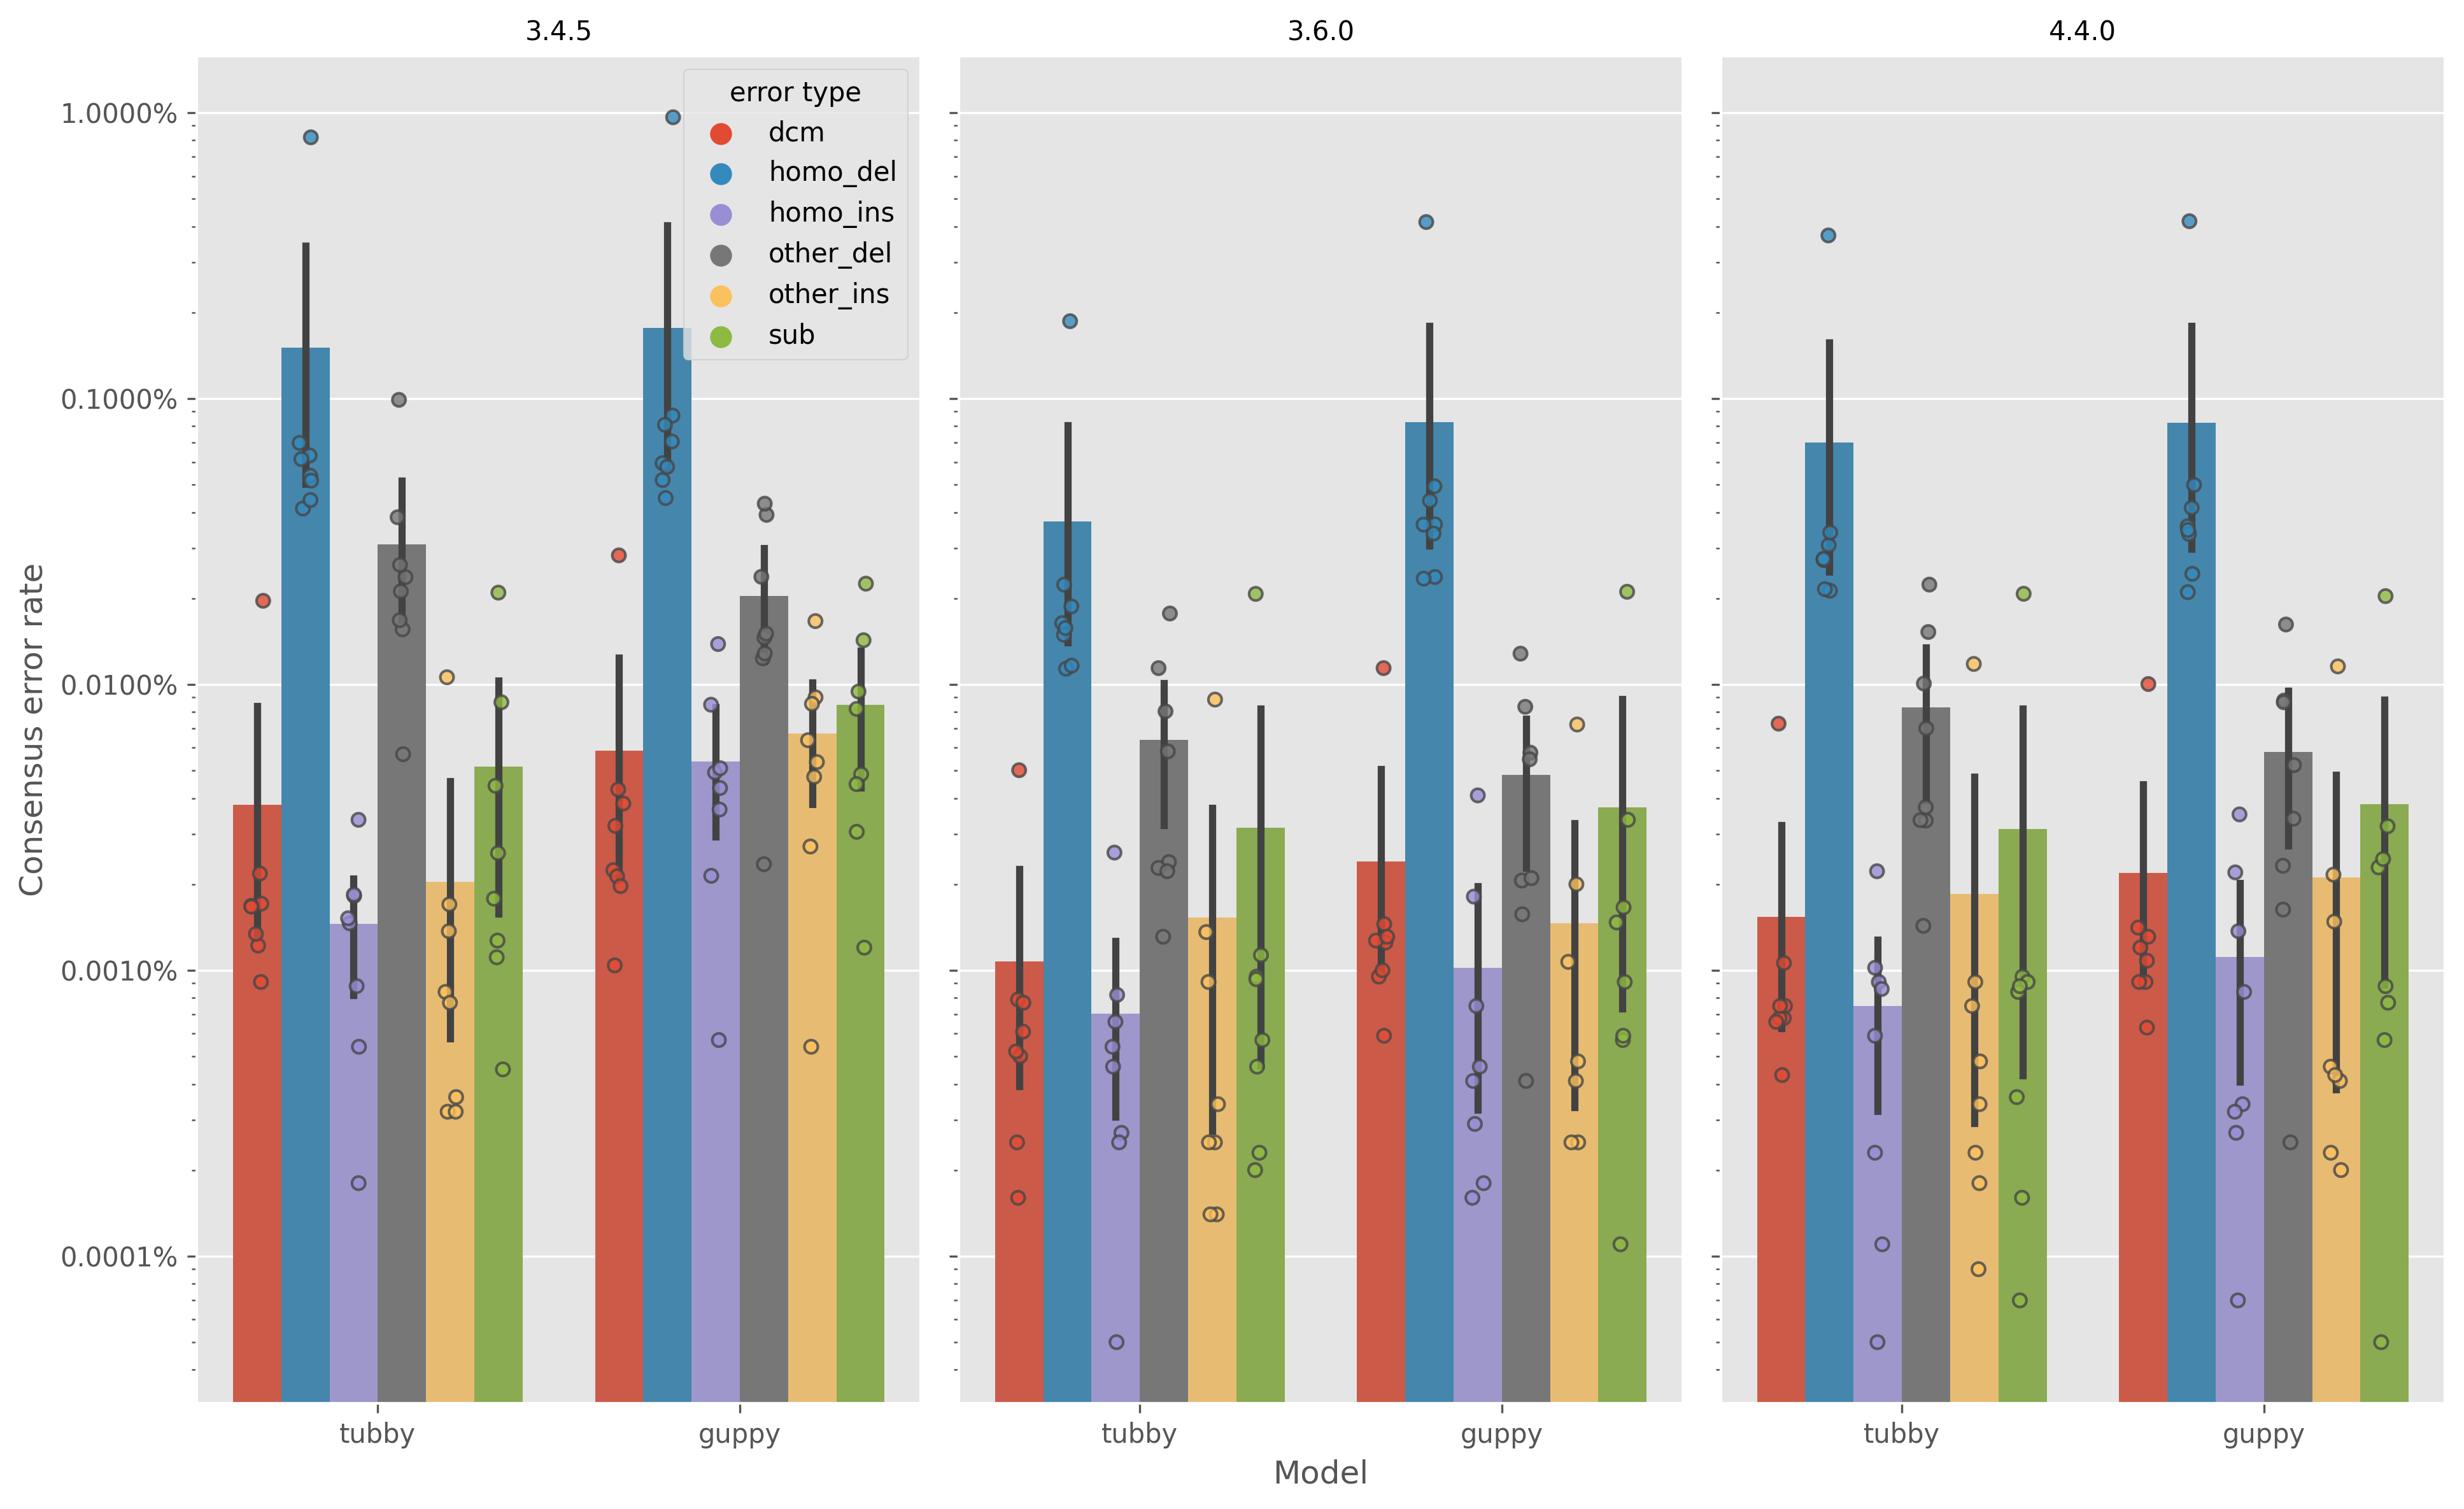
\includegraphics[width=1.0\textwidth]{Chapter4/Figs/eval_error_types.png}
        \centering
        \caption{Validation data}
        \label{fig:eval-error_types}
     \end{subfigure}
     \hfill
     \begin{subfigure}[b]{0.9\textwidth}
         \centering
        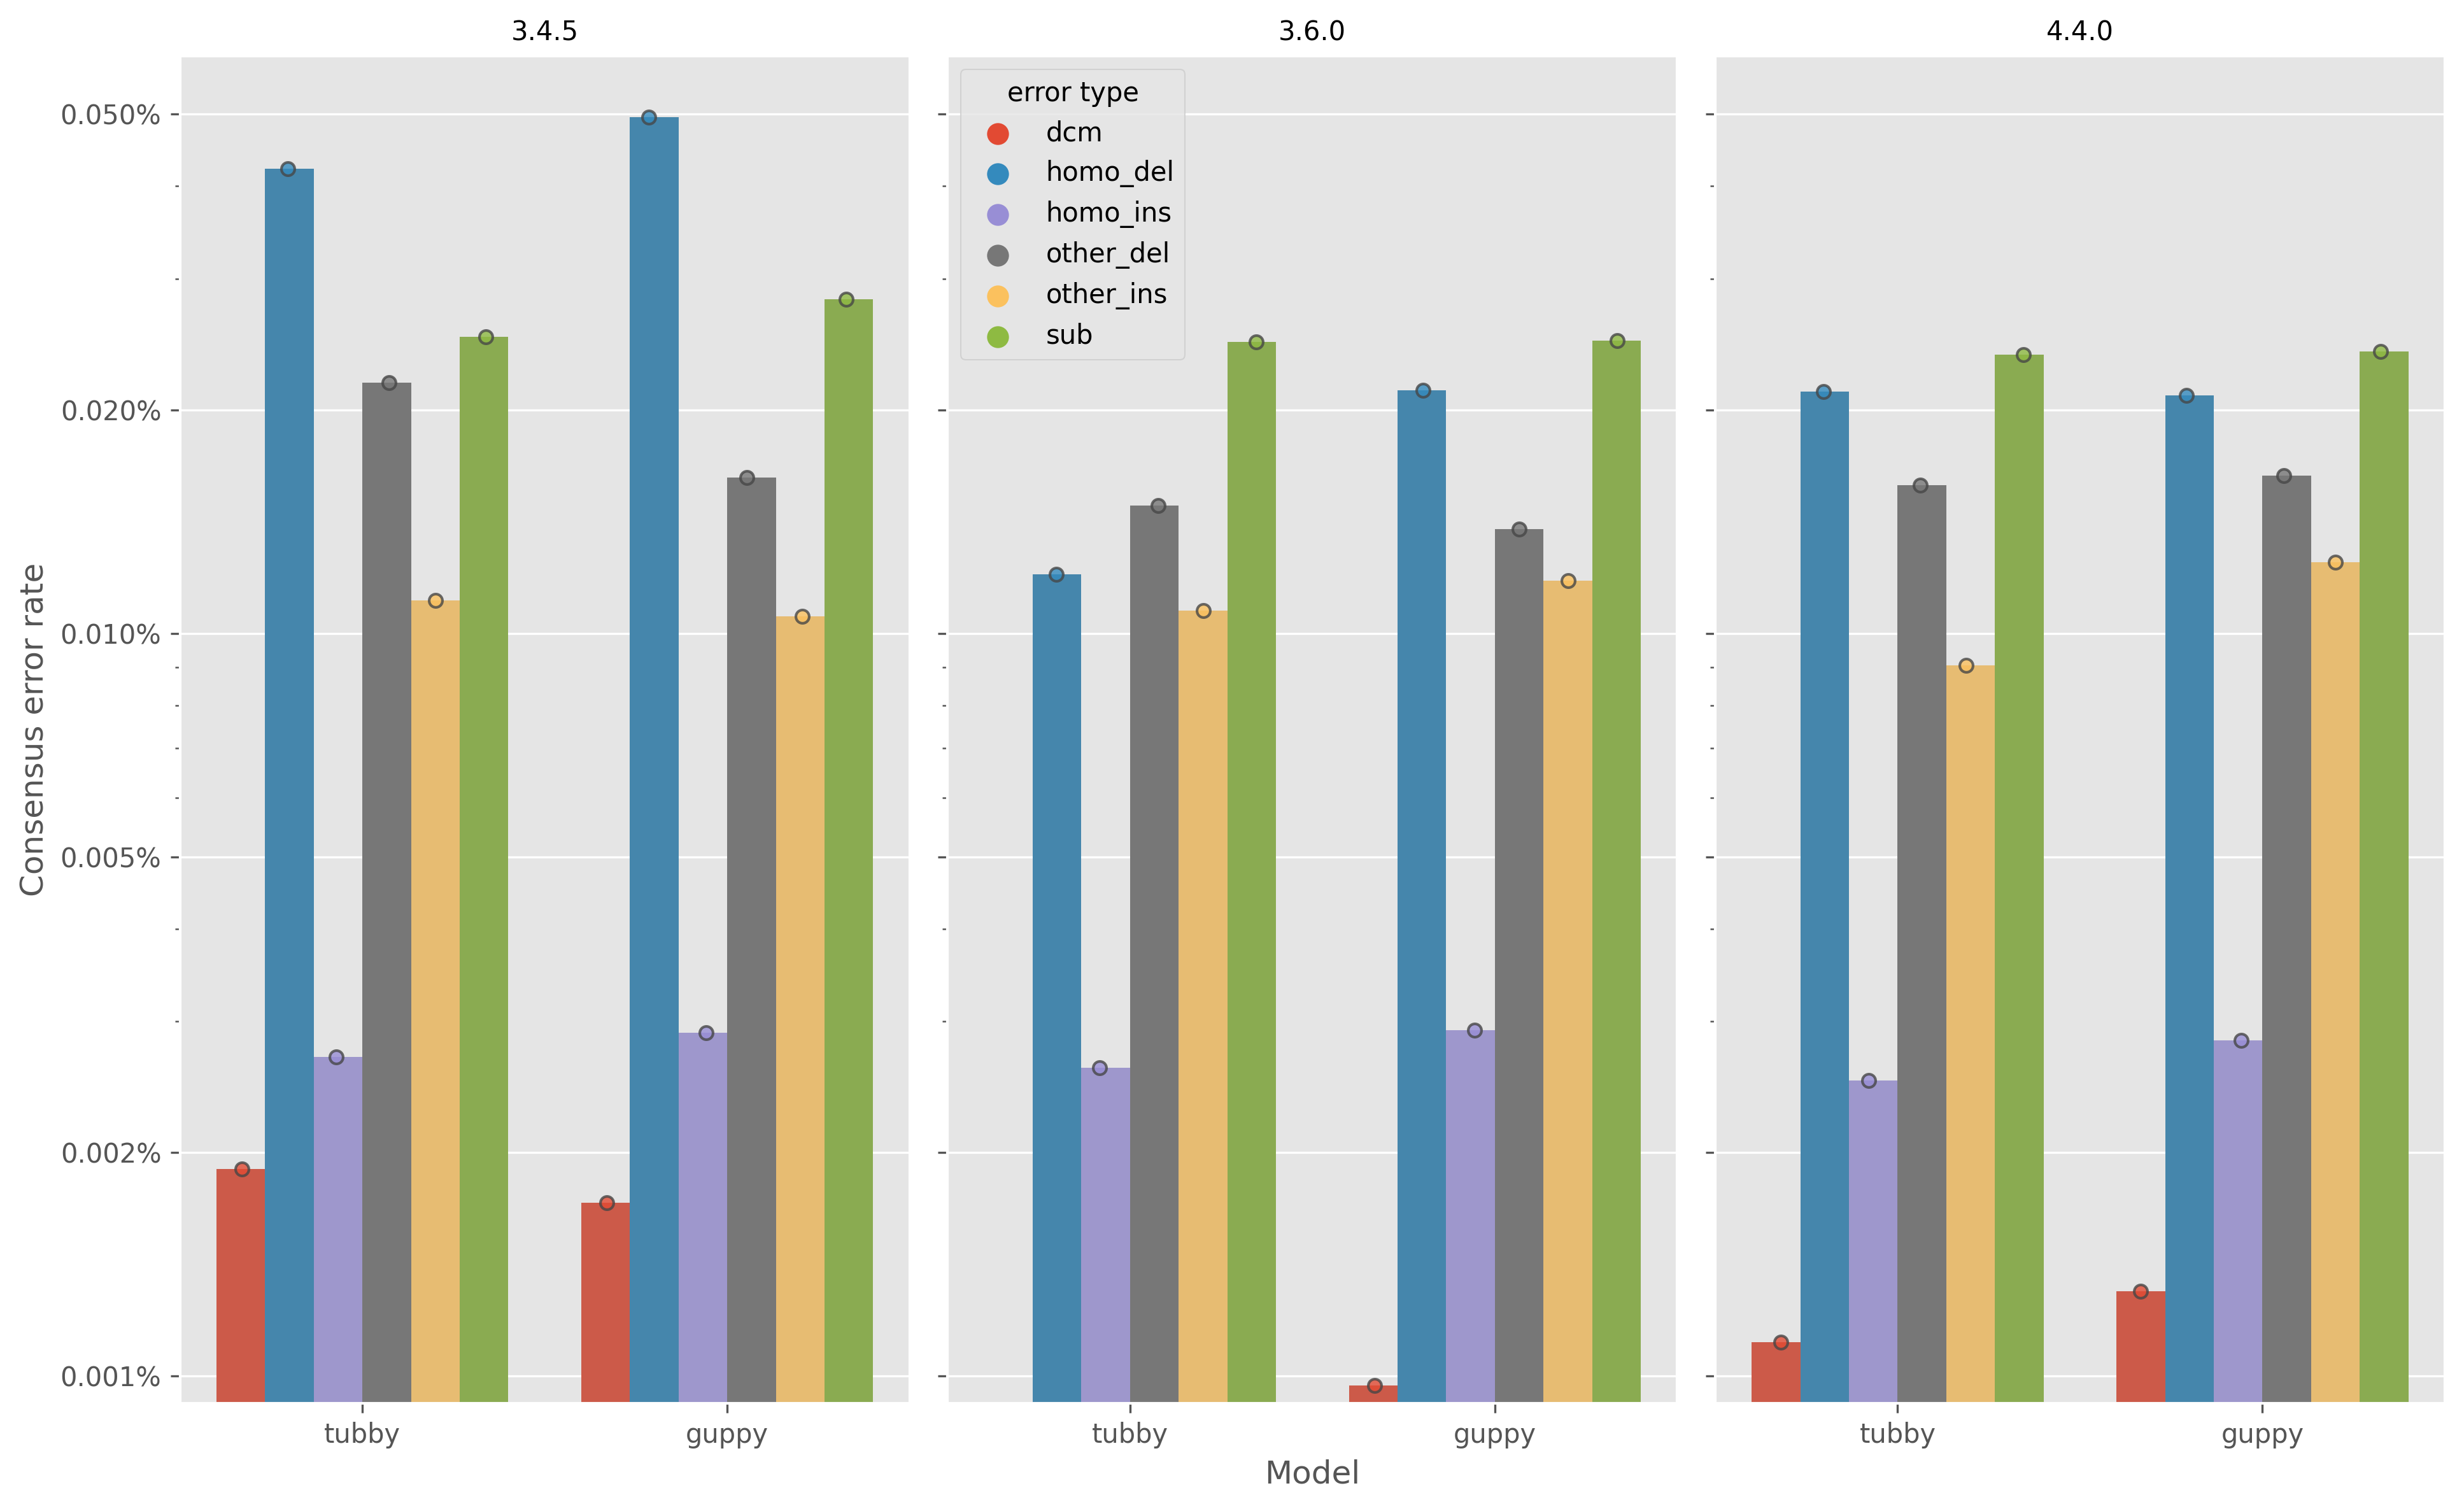
\includegraphics[width=1.0\textwidth]{Chapter4/Figs/test_error_types.png}
         \caption{Test data}
         \label{fig:test-error_types}
     \end{subfigure}
        \caption{Error types in the \vrb{rebaler} assemblies produced from reads basecalled with \tubby{} and default \guppy{} basecalling models. The consensus error rate is the number of errors attributable to that error type divided by the length of the truth assembly. The errors are per-assembly, so the confidence intervals represent variation in error types between samples/assemblies, with the points showing each assembly's value. dcm (red) refers to Dcm-methylation motifs. homo refers to homopolymer insertions (purple) or deletions (blue). other refers to non-homopolymer insertions (yellow) or deletions (grey). sub (green) is substitutions (single- or multi-base).}
        \label{fig:error_types}
\end{figure}

\subsubsection{Test data}

\autoref{fig:test-error_types} shows the error types for the BCG test sample. Interestingly, for versions 3.6.0 and 4.4.0, we find substitutions are the most common form of error; in contrast to homopolymer deletions being the overwhelming most common in the validation data. However, we do note that the test sample is a single sample, whereas the evaluation data is from eight samples.

\tubby{} version 3.6.0 has the lowest homopolymer deletions error rates, and the lowest overall error rate (0.0656\%) compared to \guppy{} (0.0755\%).

%%%%%%%%%%%%%%%%%%%%%%%%%%%%%%%%%%%%%%%%%%%%%%%%%%%%%%%%%%%%%%%%%%%%%%%%%%%%%%%%%
\section{Discussion}

The accuracy of any sequencing data has flow-on effects in almost all meaningful bioinformatics applications. We have explored a number of these in \autoref{chap:denovo}, \autoref{chap:clustering} and \autoref{chap:dst} of this thesis, with most of the focus being on \ont{} data. In this chapter, we trained a \mtb{}-specific \ont{} basecalling model, \tubby{}, which improves the accuracy of ONT's basecalling software \guppy{} for both read- and consensus-level identity.

Wick \etal{} were the first to show that training a \ont{} basecalling model for a specific taxon leads to increased accuracy \cite{wick2019}. Indeed, their work has stood as a valuable resource for the comparison of basecalling methods and the temporal improvement of \ont{} sequencing error rates. While their taxon of interest  was \textit{K. pneumoniae}, we also find the same accuracy improvements over the default methods as a result of training specifically for \mtb{}.

The most striking difference between the results obtained by Wick \etal{} and those in this chapter are the advancement in basecalling accuracy in the space of two years. The latest \guppy{} version tested by Wick \etal{} was version 2.2.3 - released in January 2019 - which yielded a median read identity of 87.15\% for the default model and 90.87\% for their taxon-specific model. In contrast, for \guppy{} version 3.6.0 - released in April 2020 - we find read-level accuracy of 94.13\% for the default model and 95.54\% for our custom \tubby{} model on the validation data. On our test data, we see even higher median identities of 95.89\% and 96.64\% respectively.

Such improvements in read identity will likely have implications in many applications. For example, \kmer{}-based methods, such as genome assembly \cite{koren2017}, read alignment \cite{li2018}, species identification \cite{Breitwieser2018}, and even variant calling (\cite{iqbal2012} and \autoref{chap:denovo}), rely heavily on error rates. To illustrate, consider the how the error rate for \guppy{} v2.2.3 (0.1285; $1-$ read identity), and \guppy{} (0.0587) and \tubby{} (0.0446) versions 3.6.0 effects the number of erroneous \kmer{}s. The equation $p=(1-e)^k$, describes the probability $p$ of a \kmer{} having \emph{no} errors, given an error rate $e$. With a commonly used \ont{} \kmer{} size is 15, \guppy{} v2.2.3 has $p=0.1271$, while \guppy{} and \tubby{} version 3.6.0 have $p=0.4036$ and $p=0.5044$ respectively. If a genome contains a given \kmer{} once, and is sequenced with no errors to a depth of 100, we would expect 100 copies. However, with the \ont{} basecalling error rates outlined, \guppy{} v2.2.3 would produce only 13 perfect copies, while \guppy{} and \tubby{} v3.6.0 would generate 40 and 50 perfect copies respectively. 

The differences between all of these basecalling models is quite stark when the impact on "lost" sequencing depth is considered this way. Focusing on the version 3.6.0 models assessed in this chapter, \tubby{} would provide 1.25x more 15-mers than \guppy{}, and 3.97x more than \guppy{} v2.2.3 reported by Wick \etal{}. This disparity in expected \kmer{} depth only increases as the \kmer{} size increase - as shown in \autoref{fig:err-rate-kmer}.

\begin{figure}
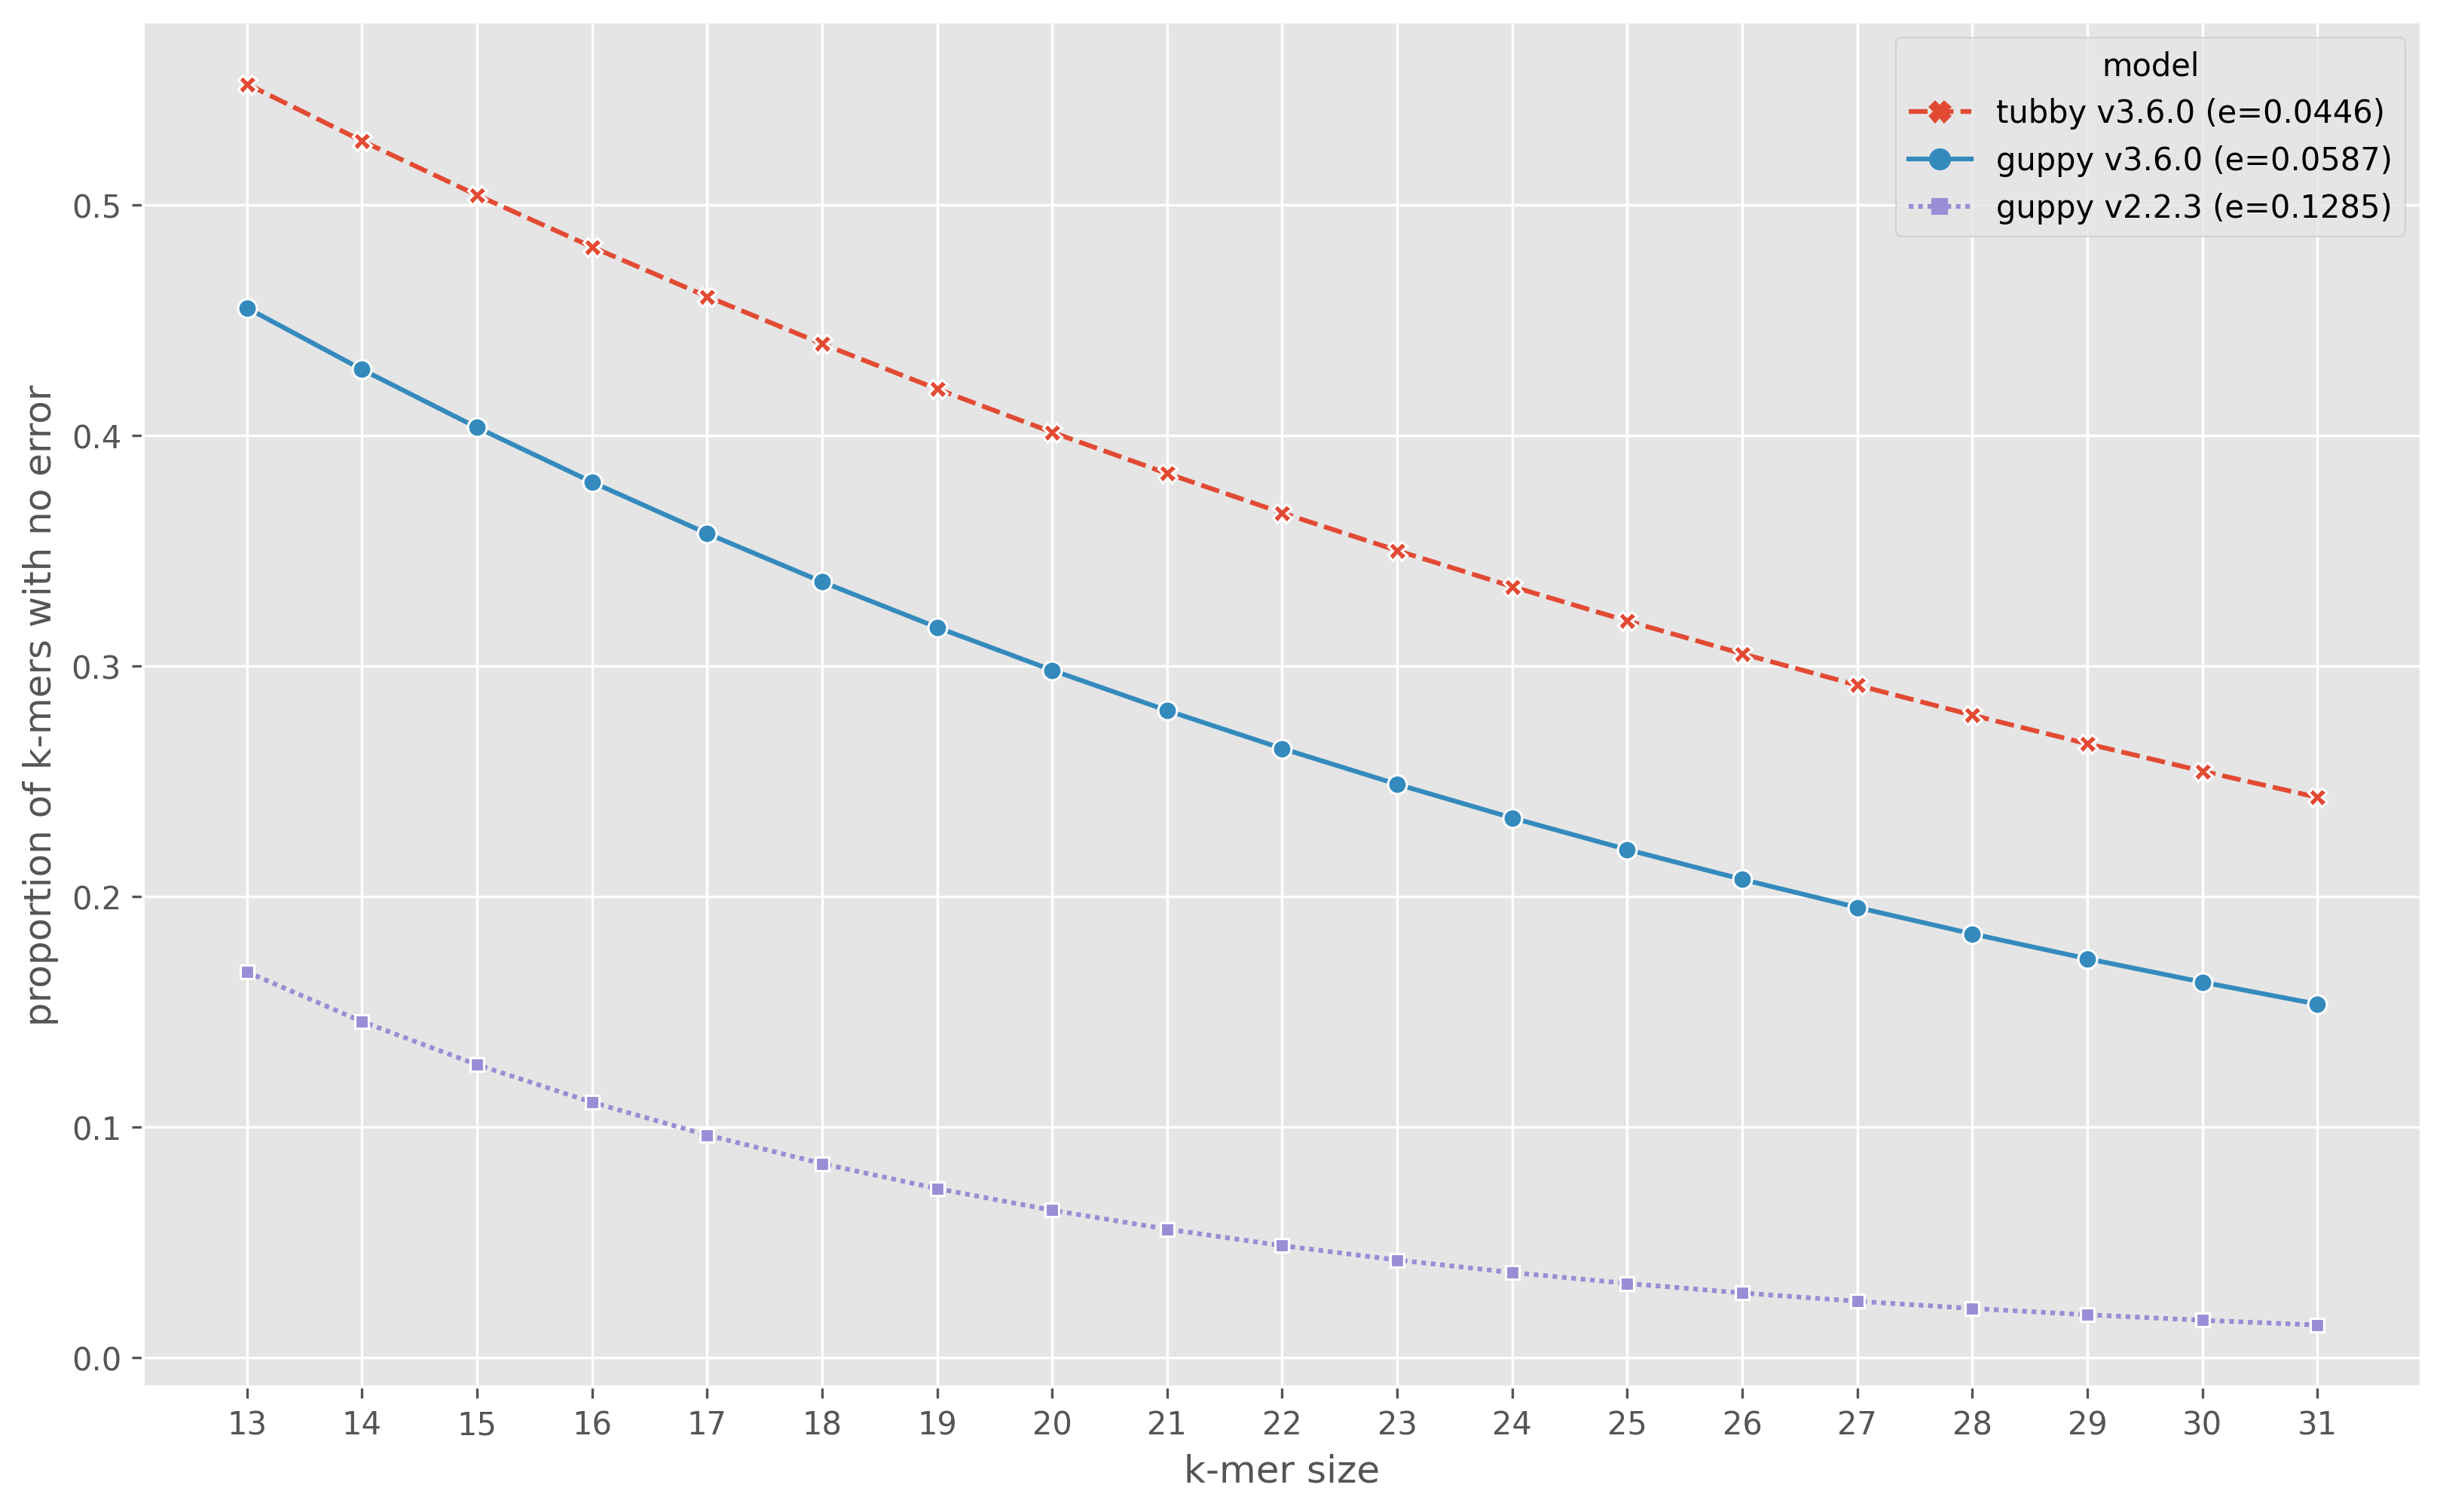
\includegraphics[width=0.9\textwidth]{Chapter4/Figs/error_rate_k.png}
\centering
\caption{Impact of error rate on expected \kmer{} depth. The y-axis shows the expected proportion of \kmer{}s with no sequencing errors for a given basecalling model (colours) with error rate, e.}
\label{fig:err-rate-kmer}
\end{figure}

An interesting observation is that for both \guppy{} and \tubby{}, the test data yielded \emph{higher} read identity values than the validation data - e.g., 1.10\% higher for \tubby{} v3.6.0. As no test data was used in the training process, this would suggest our model generalises well. However, we caution that our test data contains only one sample. Future work would benefit from increasing the number of test samples to consolidate this result.

\noindent
We chose to assess consensus accuracy in two ways to balance the strengths and weaknesses of each. The chromosome identity, as used by Wick \etal{} in 2020 \cite{wick2020}, which provides a single value for each contig, is useful for gaining a sense of the reliability of the assembly produced from the \ont{} reads as a whole. However, one weakness of this approach is if there are a small number of large erroneous regions, the overall metric is impacted. The downside here is that you may lose sight of how well the rest of the genome is assembled. A perfect example of this is the \ppe{} genes in \mtb{}, which can have a GC-content as high as 80\%, and even short reads generally fail to accurately recreate these regions \cite{Phelan2016}. To counteracts this, we also calculate the consensus BLAST identity, as-per Wick \etal{} in their 2019 bascaller comparison work mentioned above. This method breaks the assembly into 10kbps pieces and aligns those to the truth genome, allowing us to calculate BLAST identity as we did for the read identity. The benefit to this approach is we get a better sense of the average accuracy of an assembly, and any erroneous regions, such as \ppe{} genes, do not have a large impact on the overall result. For applications where repetitive and GC-rich regions are masked, this metric is a fairer guide than the overall chromosome identity.

In terms of the chromosome identity, \tubby{} v3.6.0 had the highest median value for the validation data (99.96\%) and the highest value for the single test data contig (99.11\%). In the case of the validation data, this was 0.02\% greater than the best \guppy{} value, equating to approximately 880 less erroneous positions. The test data difference was a massive 0.25\% (11,000 positions) difference between \tubby{} and \guppy{}. It is worth noting that these consensus assemblies are reference-guided, so comparisons to work such as \cite{wick2020} are not valid.

When assessing the consensus BLAST identity, we again find that \tubby{} version 3.6.0 has the highest median value for both the validation and test data. As we used the same method as Wick \etal{} in their basecaller comparison work, we can compare our results to theirs. Doing this, we see the same trend as the read-level identity; consensus accuracy has increased dramatically in the last two years. Additionally, our taxon-specific basecalling model leads to even further improvements, as did theirs. 

Comparing the latest version used by Wick \etal{}, \guppy{}'s default model has improved from a v2.2.3 (Jan. 2019) median of 99.47\% to our 99.97\% in v4.4.0 (Dec. 2020) - 22,000 less erroneous positions in an \mtb{} genome. However, we did not see the dramatic gain in a taxon-specific model they did. For \guppy{} v2.2.3 they saw the consensus identity increase to 99.93\% (+0.46\%), whereas we only found a 0.01\% increase to 99.98\%. Although, any improvement in consensus identity is valuable, especially when the percetage is nearing 100. Even an increase of 0.01\% leads to 440 less erroneous positions in an \mtb{} genome.

\noindent
The improved results from a species-specific basecalling model are not surprising given the previous work by Wick \etal{} \cite{wick2019}. However, it does raise the question of what data is used to train the default \guppy{} models. Information about the species used is not readily available to users, which is disappointing given the impact this clearly has on the results. As we have seen, the most recent \guppy{} version did not yield the highest accuracy, leading us to wonder whether there was a shift in the species and abundances used for training in the more recent version.

While we appreciate that training a general model with all knowns species is not possible, providing a list of those being used would alert users to whether their species of interest might requires a taxon-specific model.

Ultimately the \ont{} community may be better served by sharing species-specific basecalling models. An important caveat here though is that regular benchmarks, like those maintained by Wick \etal{} \cite{wick2019,wick2020}, would be necessary whenever a new \guppy{} version is released. 

\noindent
Indels have always been a known systematic issue in \ont{} data \cite{watson2019}, with the predominant problem being homopolymer deletions and methylation sites \cite{wick2019,jain2018}. In \autoref{sec:tubby-error-types}, we found the most common error types were homopolymer deletions (and substitutions in the test data). Importantly, \tubby{} v3.6.0 reduced the number of homopolymer deletions by nearly half. This reduction is the same as Wick \etal{} when comparing their taxon-specific model to the default \guppy{}. 

As Wick \etal{} used \textit{K. pneumoniae}, which has active 5-methylcystosine methyltransferases, their major source of errors with the default \guppy{} model was Dcm methylation sites. However, training the taxon-specific model removed nearly all of those errors. \mtb{} does not have the same methyltranferases, and so Dcm methylation sites were not an issue.

We did not see any reduction in substitutions or other types of indels using \tubby{}, indicating these errors may originate from a source other than the basecaller, such as the pore itself.

\noindent
The two main limitations for the work in this chapter were that we only have one test sample and that we did not assess how the basecaller improvements impact applications outside of assembly. We discuss these further in \autoref{sec:tubby-fw}.


%%%%%%%%%%%%%%%%%%%%%%%%%%%%%%%%%%%%%%%%%%%%%%%%%%%%%%%%%%%%%%%%%%%%%%%%%%%%%%%%%
\section{Conclusion}
In conclusion, the work in this chapter shows that an \mtb{}-specific \ont{} basecalling model yields higher read- and consensus-level accuracy than default \guppy{} models. Additionally, the \mtb{} model reduces the main source of \ont{} errors - homopolymer deletions.

We trained and compared models for three \guppy{} versions. Surprisingly, the most recent version did not yield the best results for \mtb{} and highlights the need for regular benchmarks of \ont{} basecalling performance.

%%%%%%%%%%%%%%%%%%%%%%%%%%%%%%%%%%%%%%%%%%%%%%%%%%%%%%%%%%%%%%%%%%%%%%%%%%%%%%%%%
\section{Future work}
\label{sec:tubby-fw}

\subsection{\denovo{} assembly assessment}
The methods we used for assessing the consensus-level accuracy of \tubby{} generated reference-guided assemblies using \vrb{rebaler}. While this helps keep the overall structure of the assemblies the same, and thus allow for focusing on the base-level accuracy, it fails to show what differences basecalling models cause on overall assembly structure.

One solution would be to also assess the consensus accuracy of \denovo{} genome assemblies generated from the \ont{} reads basecalled with each model. Such an analysis is similar to Wick \etal{} (2020), and could also assess other metrics like contiguity of assemblies \cite{wick2020}.

\subsection{\mtb{} methylation sites}
The major cause of \guppy{} basecalling errors in Enterobacteriaceae are Dcm methylation motifs \cite{wick2019}. While \mtb{} does not show evidence for these sites (\cite{Danjuma2017} and \autoref{sec:tubby-error-types}), it would be enlightening to see what impact \mtb{}-specific methylation sites have on the error rate. As such, future versions of this model benchmark could include such \mtb{}-specific methylation motifs \cite{chiner2019,modlin2020}.

\subsection{Impact on previous work}
While we have shown in this chapter that an \mtb{}-specific basecalling model improves accuracy and reduces homopolymer deletions, it remains to be seen what impact such advances have on "real-world" applications. \autoref{chap:clustering} and \autoref{chap:dst} of this thesis use \ont{} data for \mtb{} transmission clustering and drug resistance prediction. One simple enough test of the utility of \tubby{} would be to rerun the analyses for those chapters with \ont{} data basecalled with \tubby{}. That way, any change in results can be directly attributed to the taxon-specific model.

\subsection{Increased diversity of data}
One of the main challenges with training a basecalling model is data. The data one trains, validates, and trains on must have a known, reliable truth genome and ideally would be free of laboratory biases too. While the number of reads we use for training and validation in this chapter were more than sufficient, they were all sequenced at a similar time by the same technician, in the same laboratory. It would be prudent to include some data in the training process that was sequenced at a separate time and ideally by different people in a different place. Additionally, including data from other species in the MTBC would likely prove beneficial as non-tuberculous mycobacteria (NTM) are becoming an ever increasing cause for concern globally \cite{Johansen2020}.

\subsection{New Conditional random field models}
As mentioned alreayd, \ont{} sequencing technology is evolving at a rapid pace. Whenever a study using \ont{} is published, it is undoubtedly out-of-date with the latest tools being used - due to no fault of the authors. At the time of writing, a new major version of \guppy{} (version 5) has been released which uses a new model format based on conditional random fields (CRFs), which use probabilistic model try segment and label data \cite{Lafferty2001} - a vital component of the basecalling process. These new models can be trained using a new (easier) process in the ONT software Bonito (\url{https://github.com/nanoporetech/bonito}).

The new CRF-based models (dubbed "super-accurate" models by ONT) are reported to provide a modal read accuracy increase of 0.5\% over the \guppy{} versions used in this chapter (\url{https://community.nanoporetech.com/posts/guppy-v5-0-7-release-note}). Therefore, updating \tubby{}'s training process for these new CRF-based models may yield an even further improvement to the accuracy report in this chapter. (However, we note this section itself will likely be out-of-date by the time it is read). 

%%%%%%%%%%%%%%%%%%%%%%%%%%%%%%%%%%%%%%%%%%%%%%%%%%%%%%%%%%%%%%%%%%%%%%%%%%%%%%%%%
\section{Availability of data and materials}

\todo[inline]{need to make tubby public prior to submission}

\tubby{} is open-source and freely available under an MIT license at \url{https://github.com/mbhall88/tubby}. The models are available under Releases in compressed JSON format. The pipelines and scripts used in this chapter are available at the same location. All analyses were run using the workflow management program \vrb{snakemake} \cite{snakemake2021}. All figures were generated using the Python libraries \vrb{matplotlib} \cite{matplotlib} and \vrb{seaborn} \cite{seaborn}.

\towrite[inline]{availability of the data if it has been deposited prior to submission}